Nach dem eigentlichen Metamodell mit den Knoten- / Kantenbeziehungen und der Knotentypenhierarchie folgt die Kantentypenhierarchie in einem eigenst�ndigen Diagramm.

\begin{figure}[htbp]
  \begin{center}
	  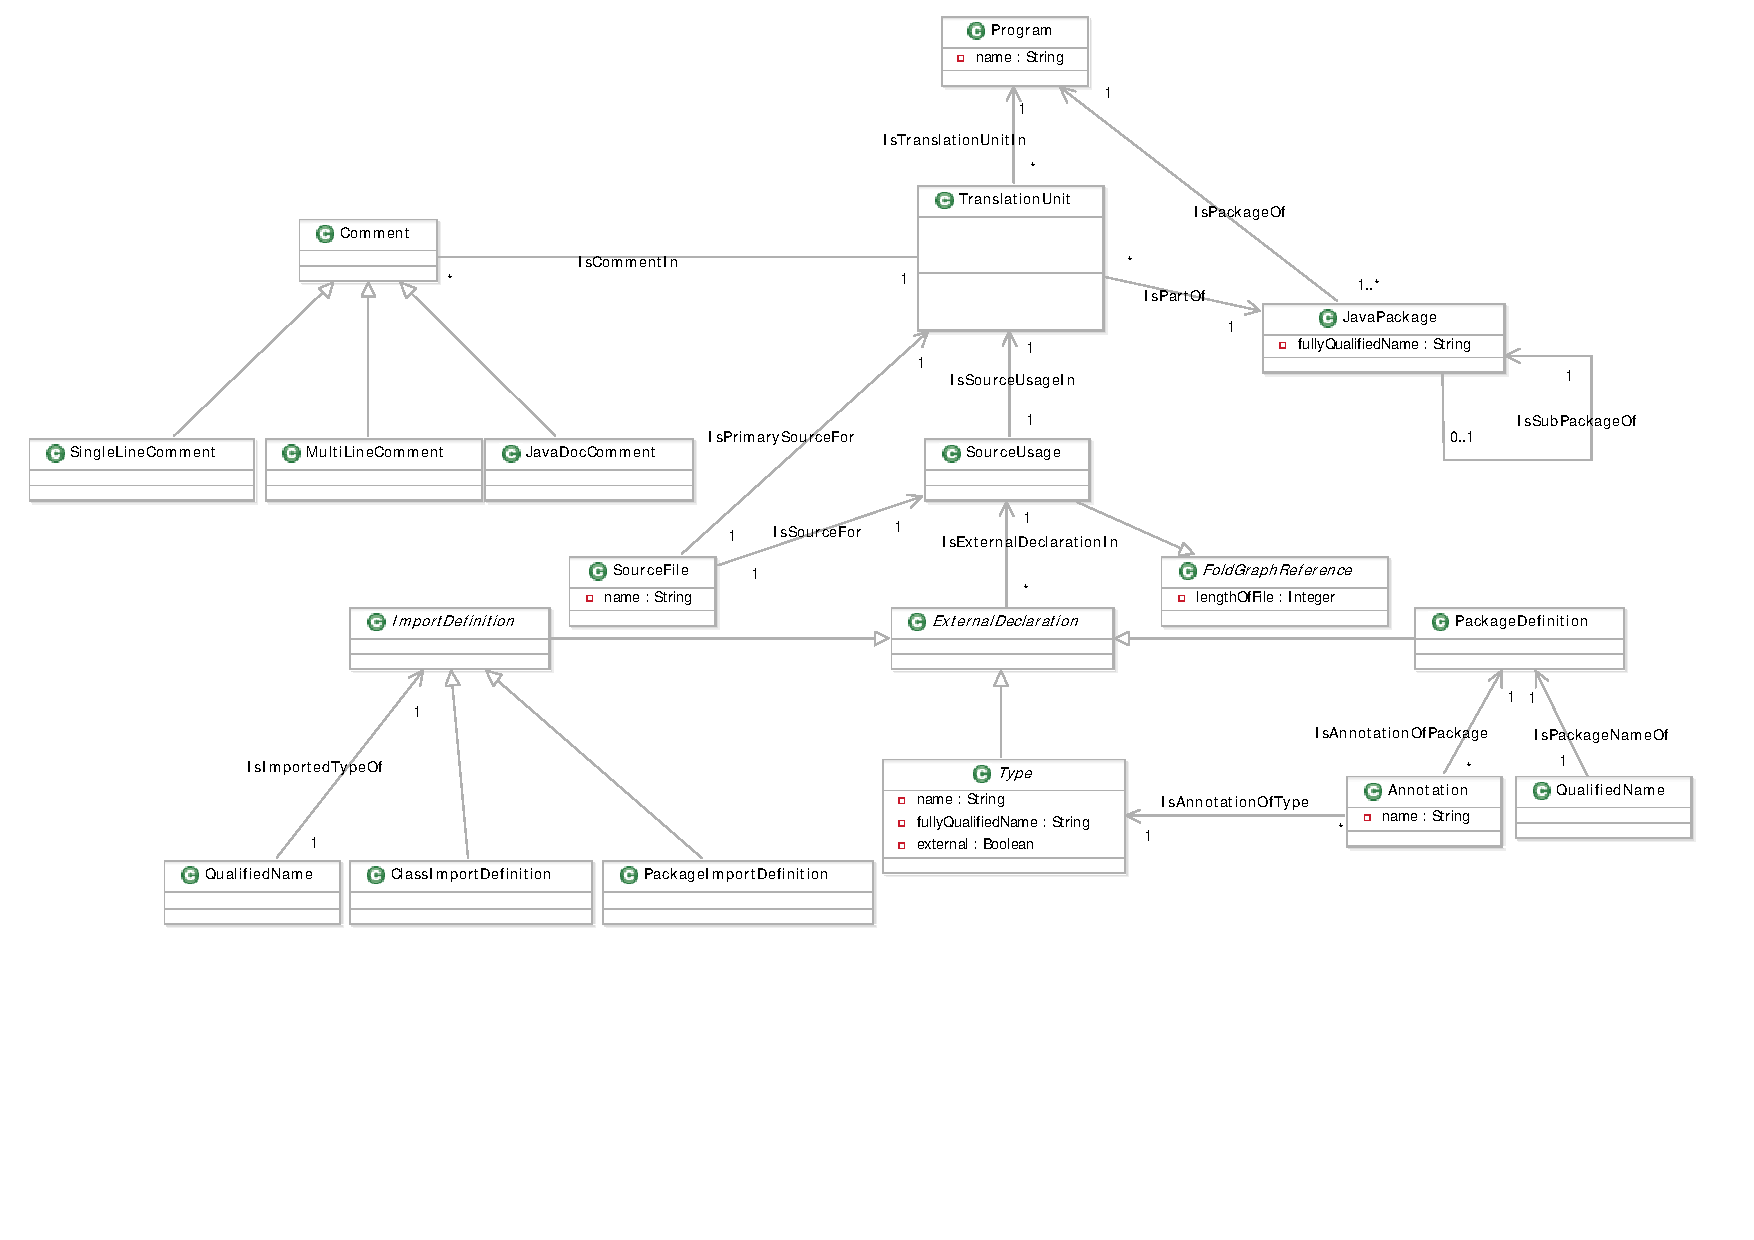
\includegraphics[width=19.8cm, angle=90]{figures/metamodell01.pdf}
	  \caption{Metamodell (Teil 1 / 12)}
  \end{center}
\end{figure}
\begin{figure}[htbp]
  \begin{center}
	  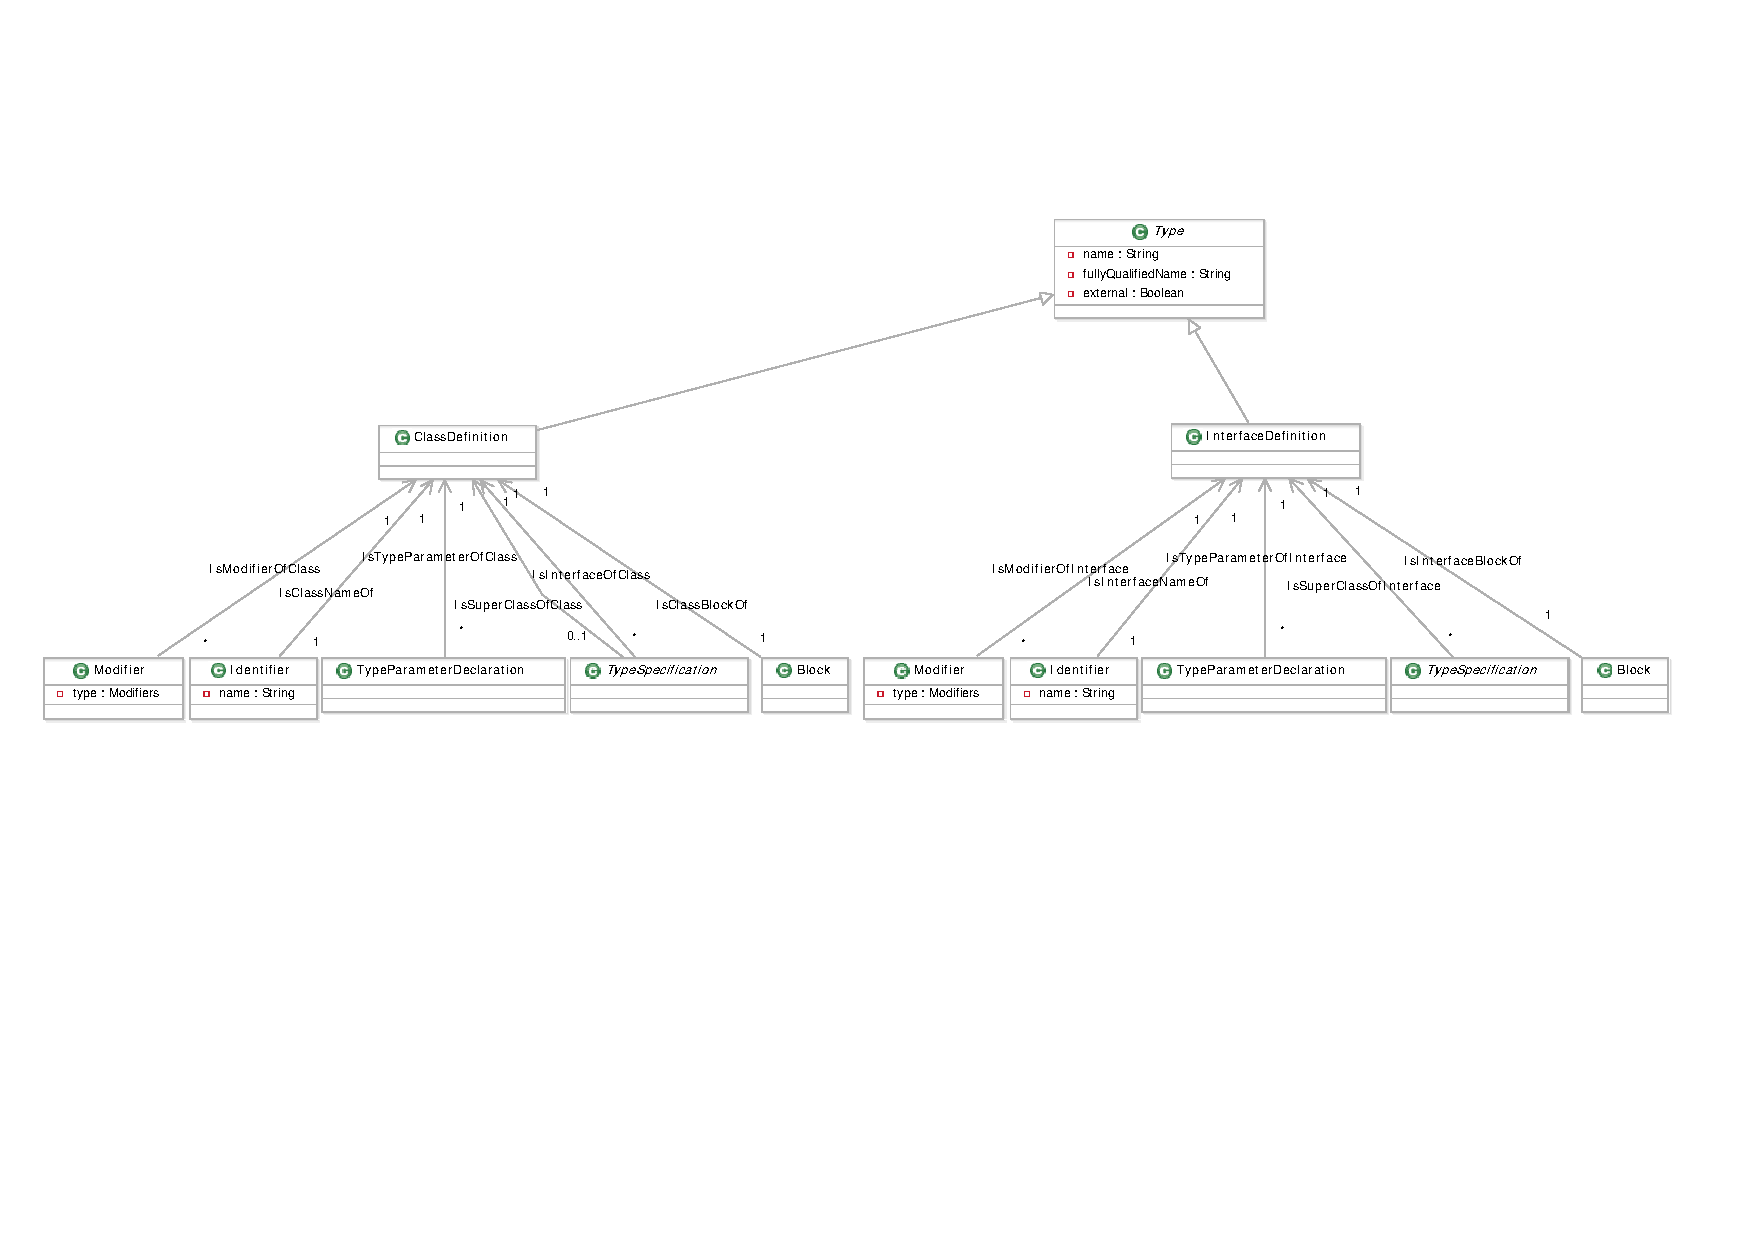
\includegraphics[width=19.8cm, angle=90]{figures/metamodell02.pdf}
	  \caption{Metamodell (Teil 2 / 12)}
  \end{center}
\end{figure}
\begin{figure}[htbp]
  \begin{center}
	  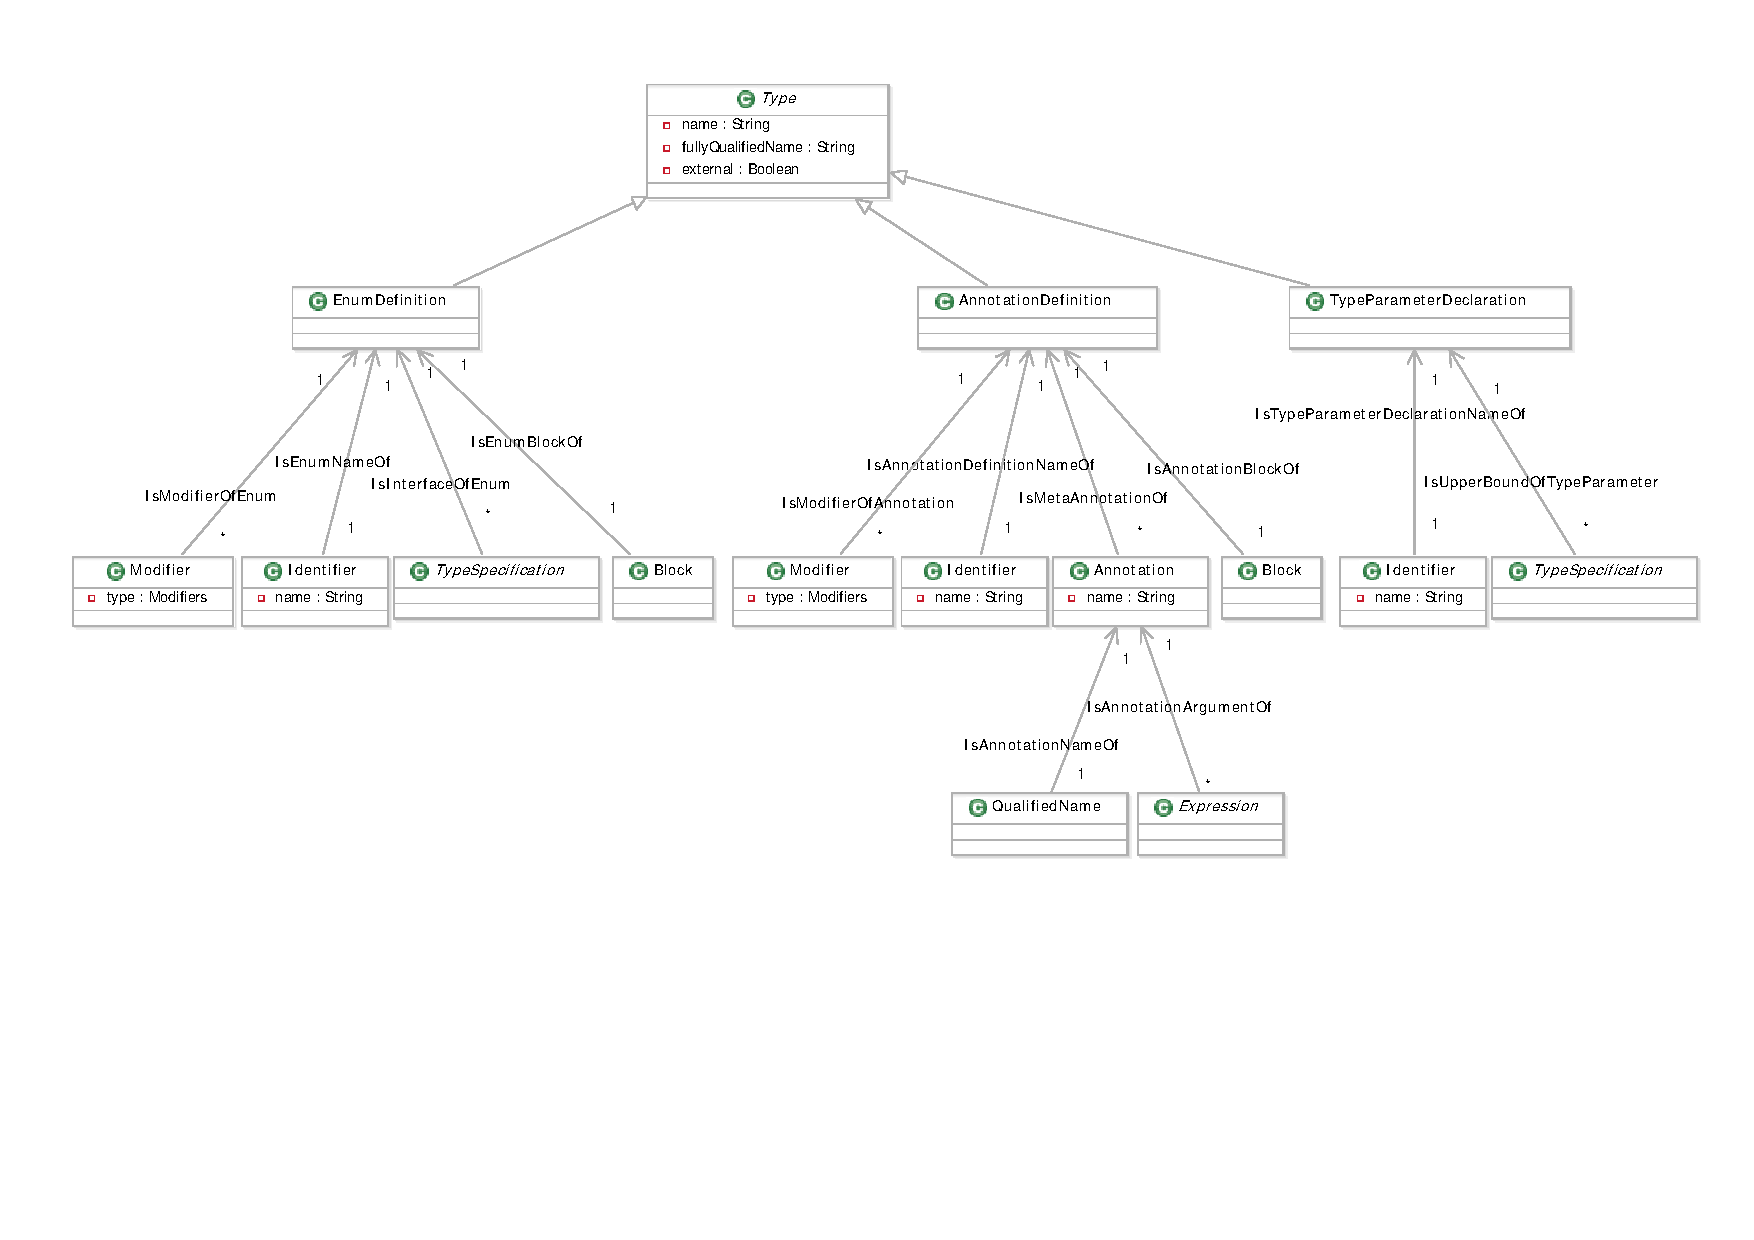
\includegraphics[width=19.8cm, angle=90]{figures/metamodell03.pdf}
	  \caption{Metamodell (Teil 3 / 12)}
  \end{center}
\end{figure}
\begin{figure}[htbp]
  \begin{center}
	  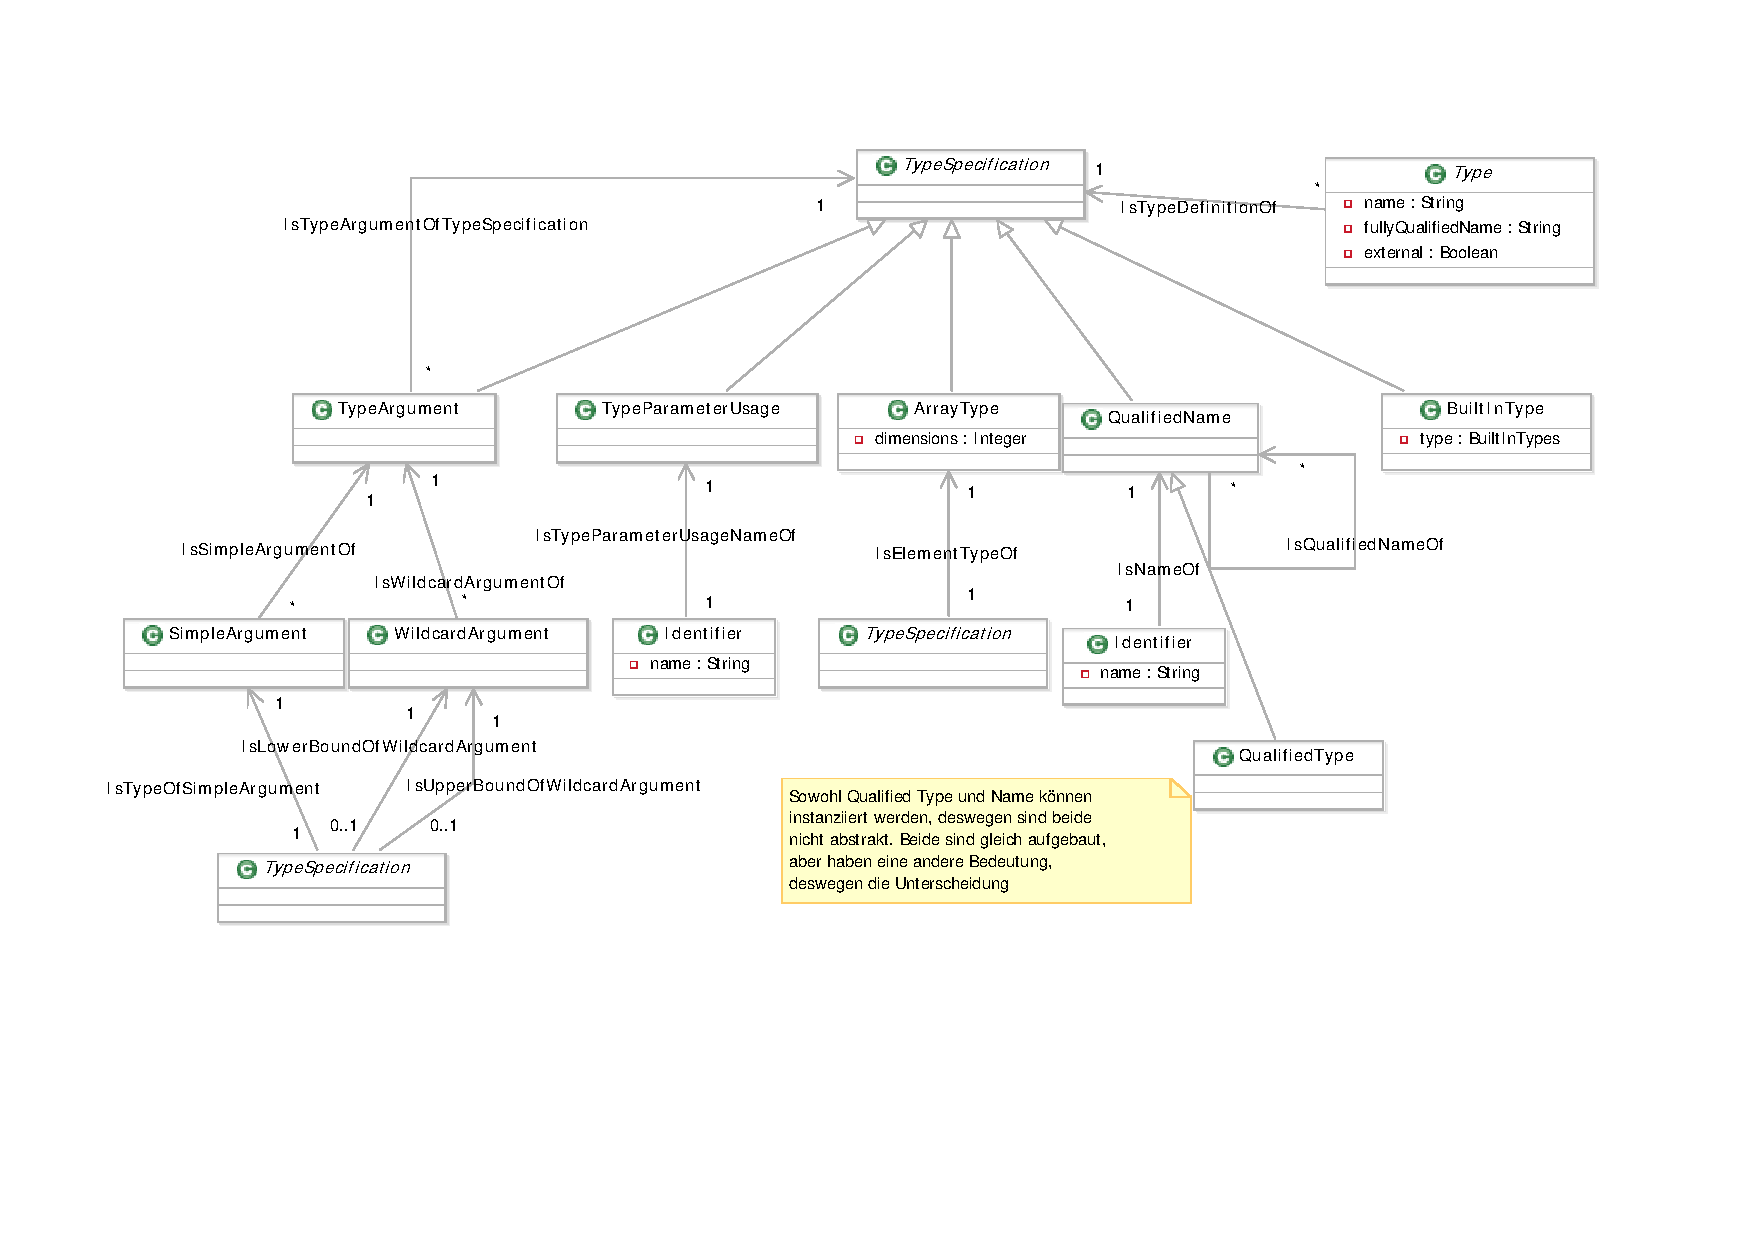
\includegraphics[width=19.8cm, angle=90]{figures/metamodell04.pdf}
	  \caption{Metamodell (Teil 4 / 12)}
  \end{center}
\end{figure}
\begin{figure}[htbp]
  \begin{center}
	  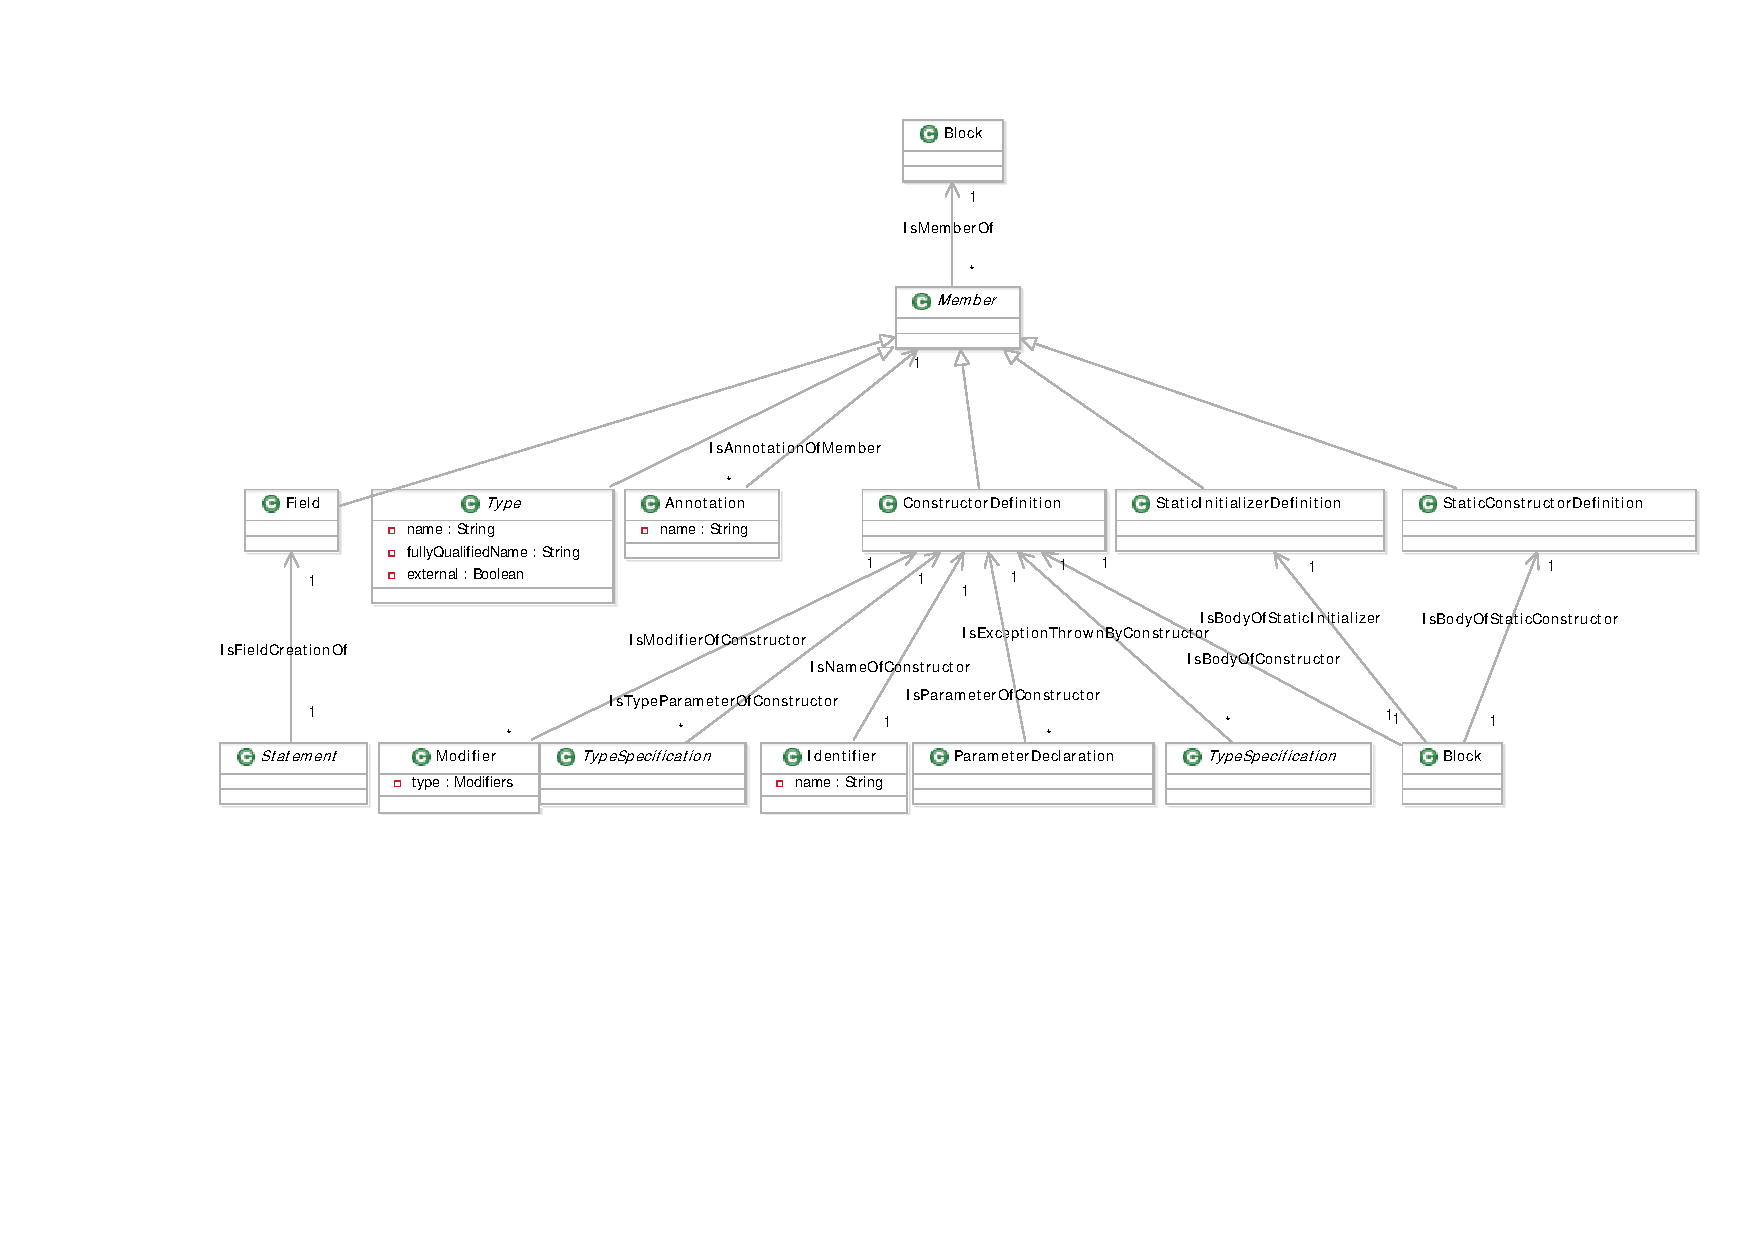
\includegraphics[width=19.8cm, angle=90]{figures/metamodell05.pdf}
	  \caption{Metamodell (Teil 5 / 12)}
  \end{center}
\end{figure}
\begin{figure}[htbp]
  \begin{center}
	  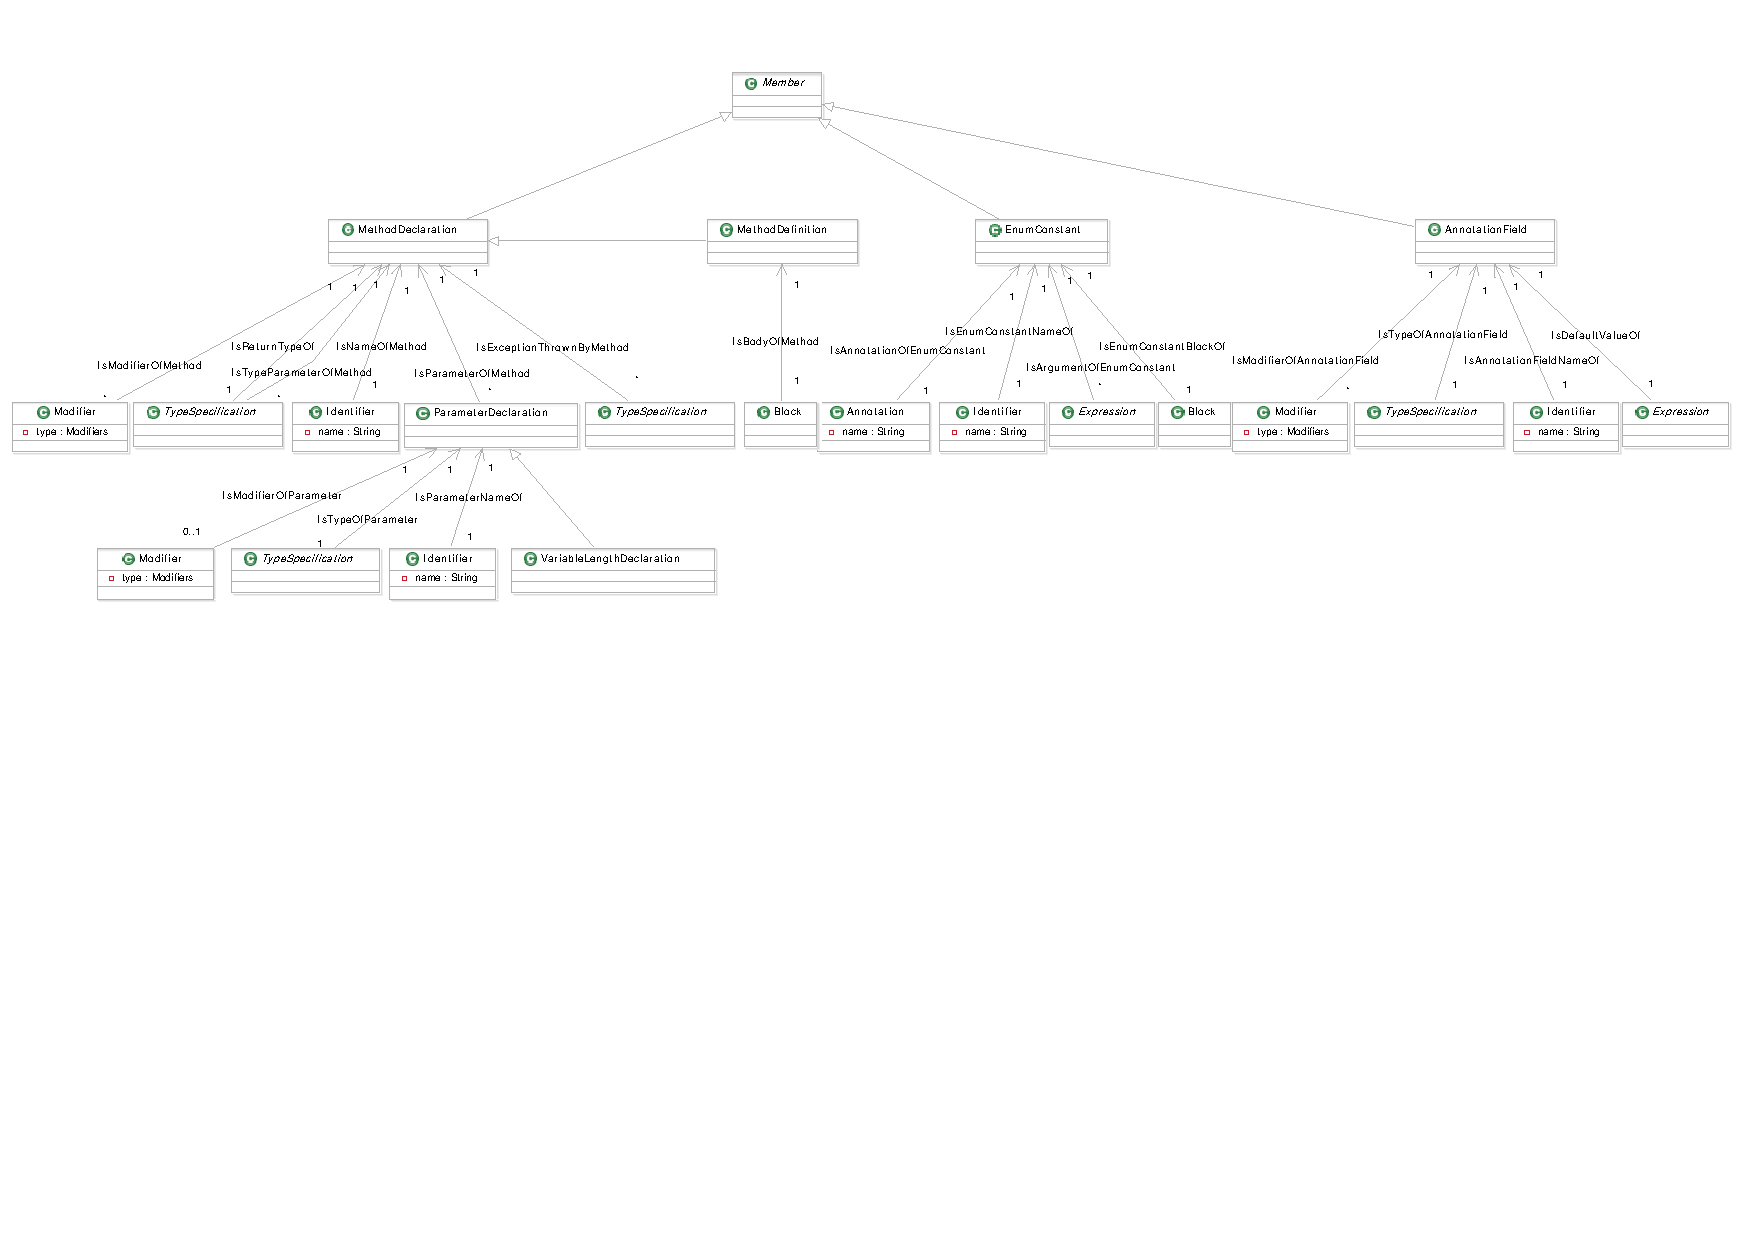
\includegraphics[width=19.8cm, angle=90]{figures/metamodell06.pdf}
	  \caption{Metamodell (Teil 6 / 12)}
  \end{center}
\end{figure}
\begin{figure}[htbp]
  \begin{center}
	  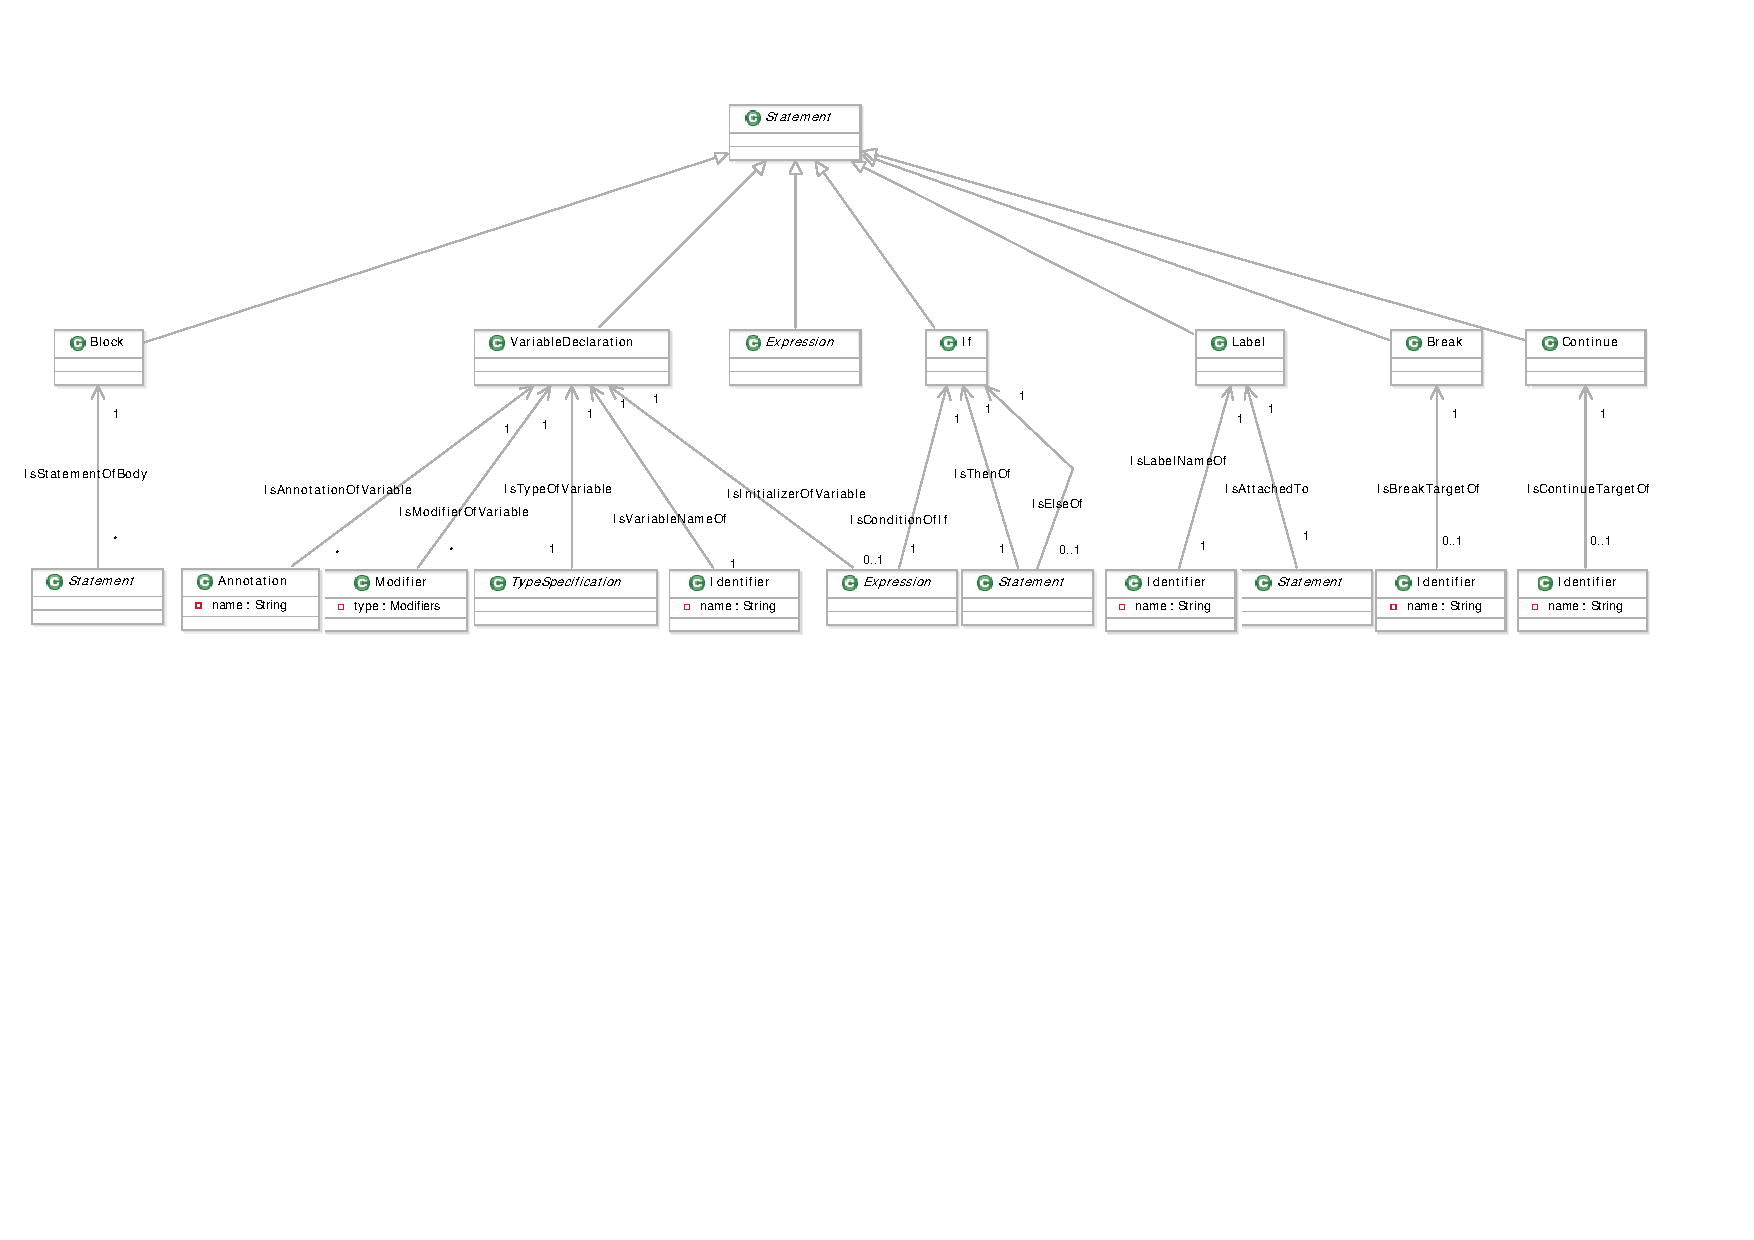
\includegraphics[width=19.8cm, angle=90]{figures/metamodell07.pdf}
	  \caption{Metamodell (Teil 7 / 12)}
  \end{center}
\end{figure}
\begin{figure}[htbp]
  \begin{center}
	  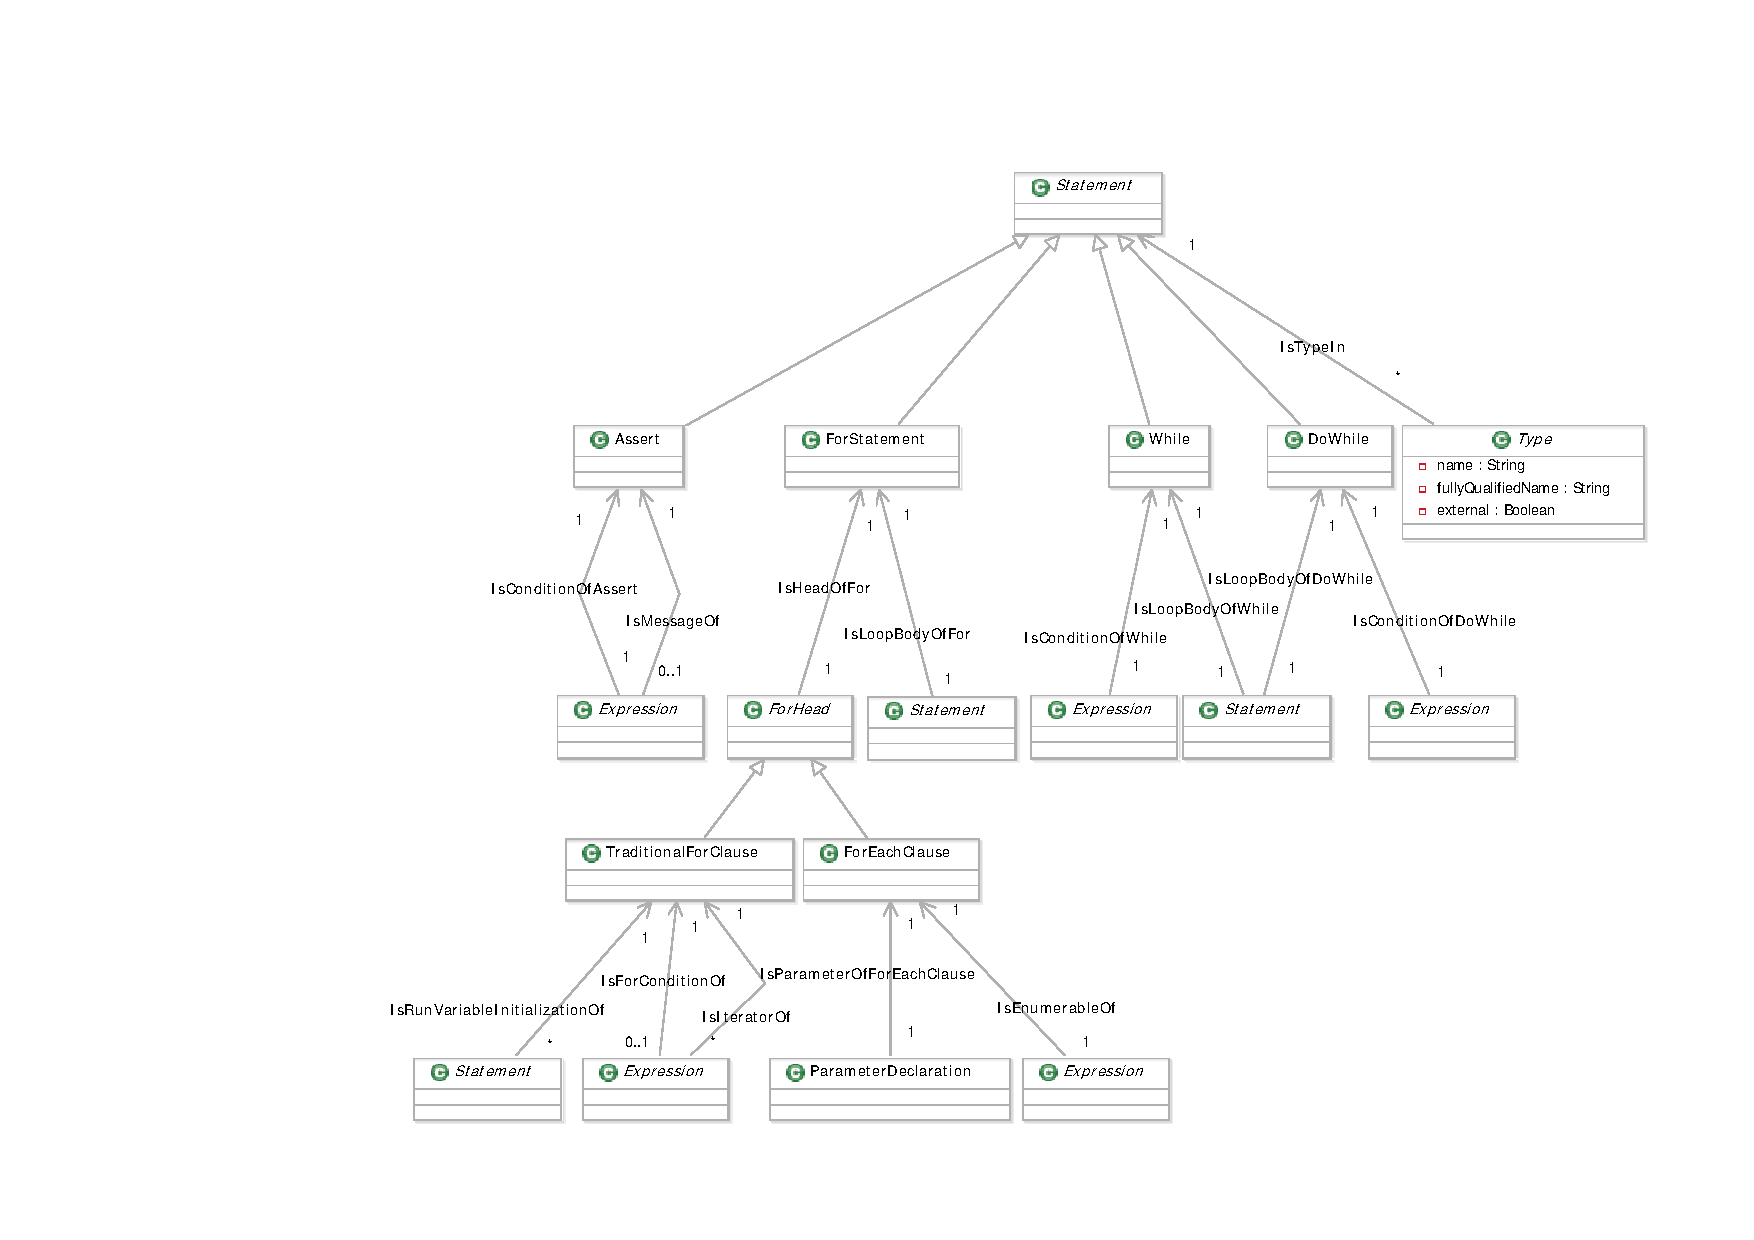
\includegraphics[width=19.8cm, angle=90]{figures/metamodell08.pdf}
	  \caption{Metamodell (Teil 8 / 12)}
  \end{center}
\end{figure}
\begin{figure}[htbp]
  \begin{center}
	  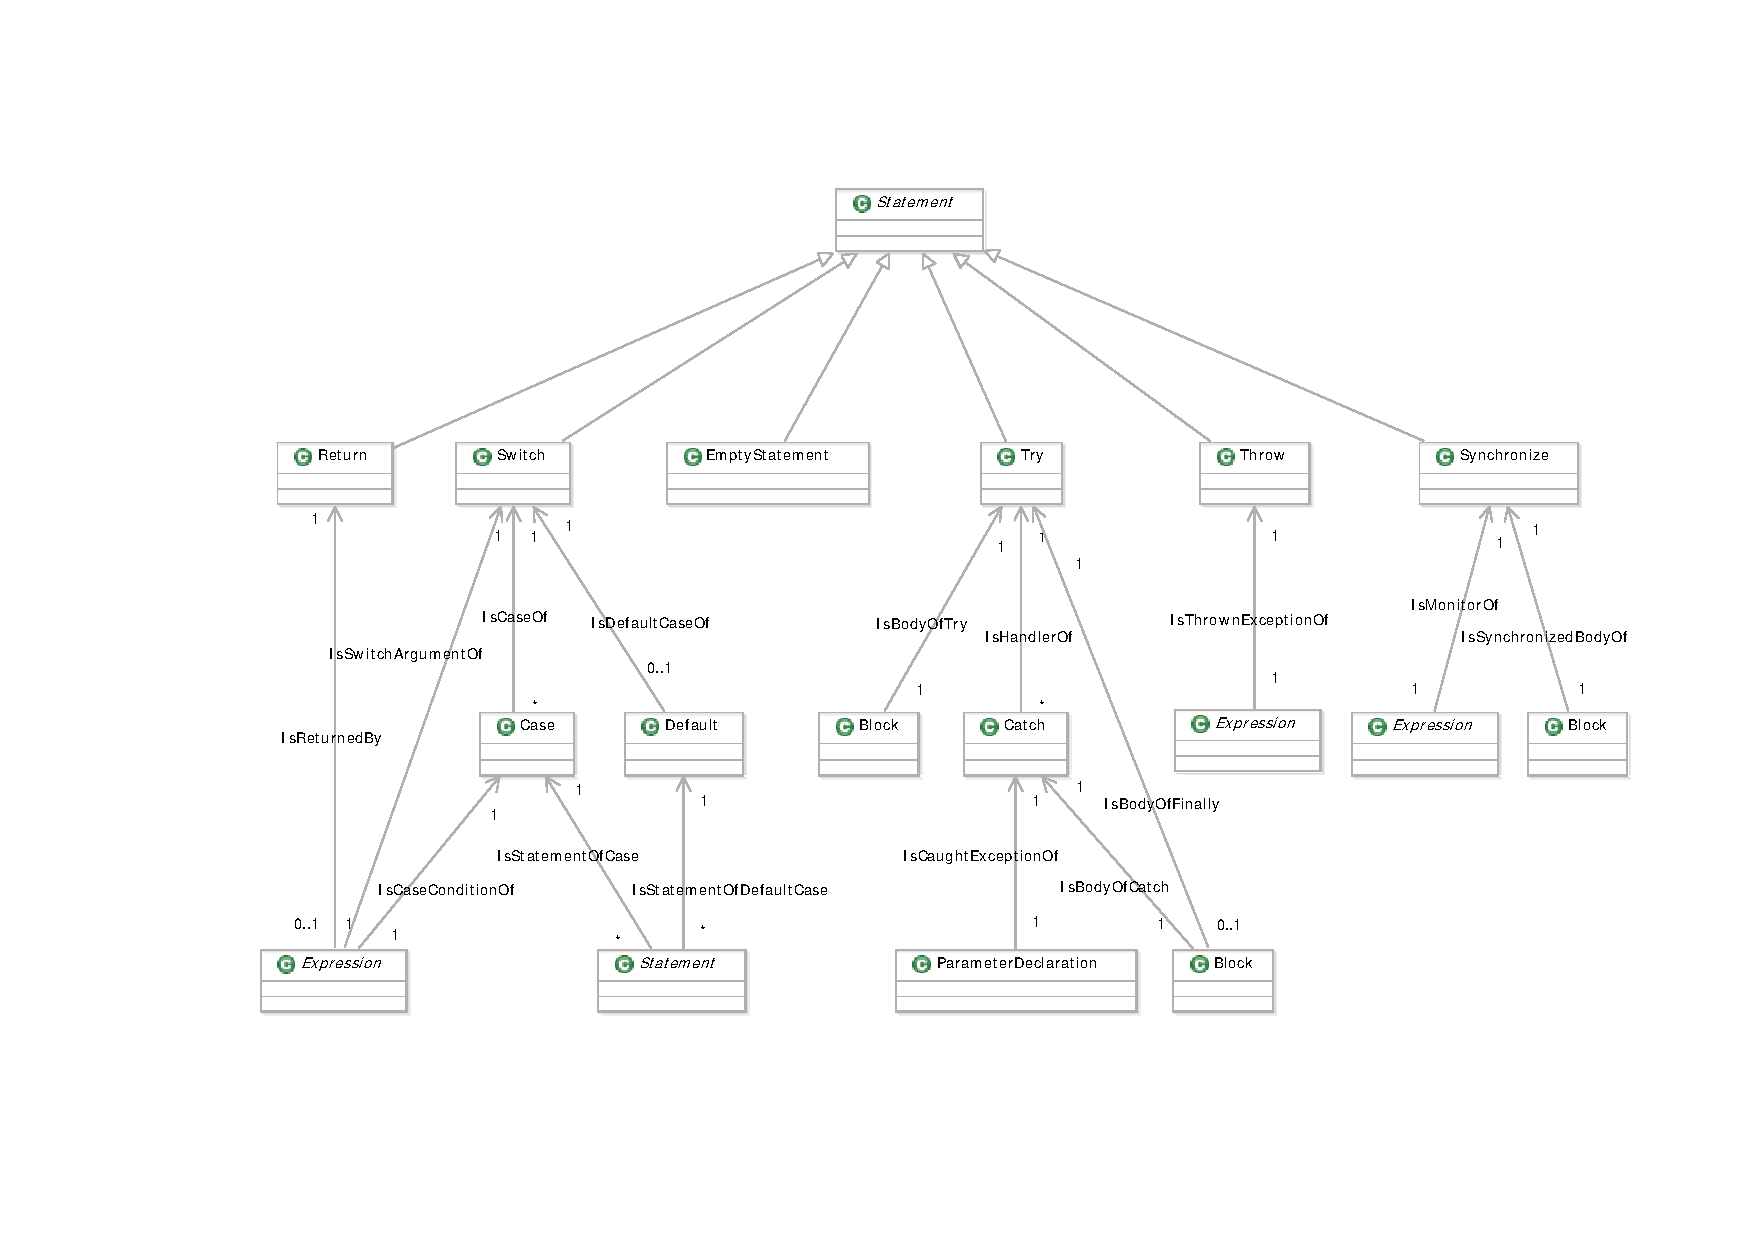
\includegraphics[width=19.8cm, angle=90]{figures/metamodell09.pdf}
	  \caption{Metamodell (Teil 9 / 12)}
  \end{center}
\end{figure}
\begin{figure}[htbp]
  \begin{center}
	  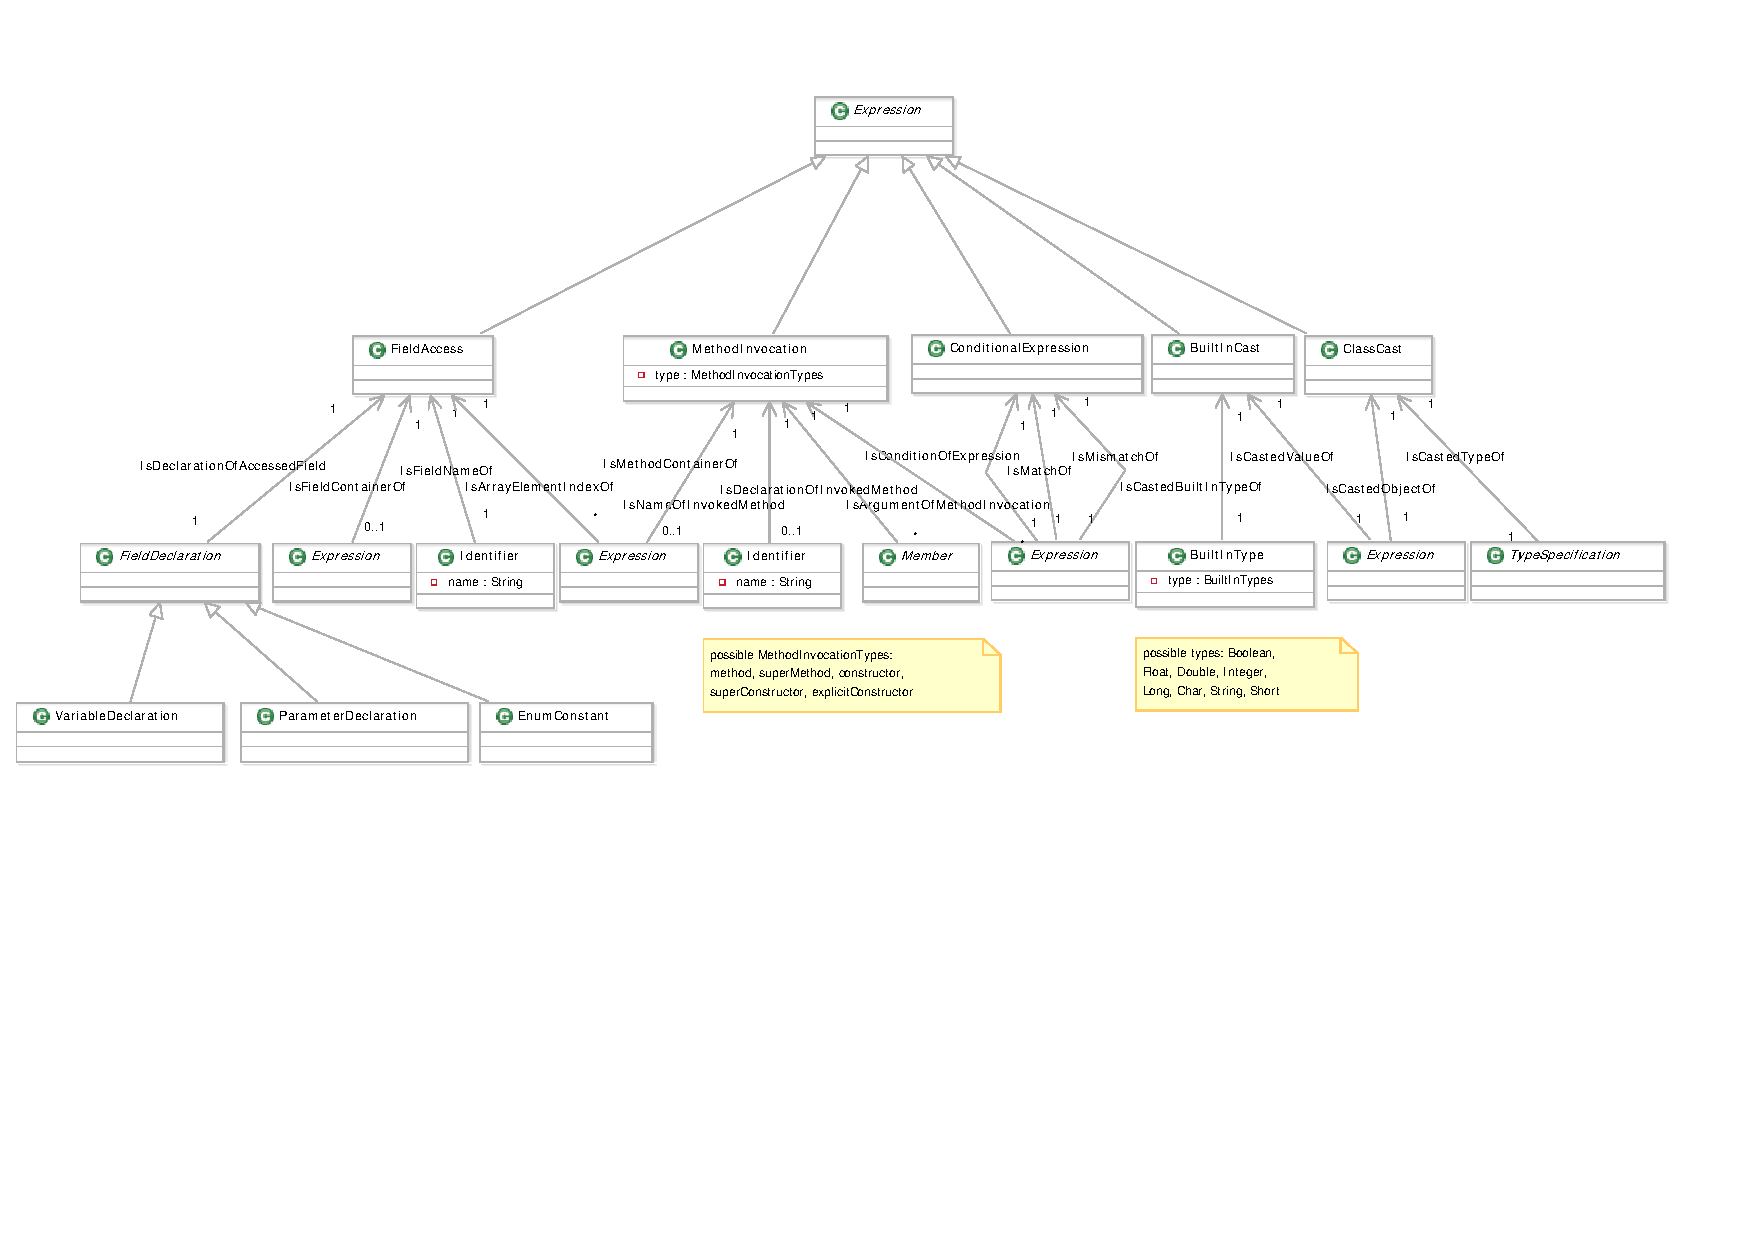
\includegraphics[width=19.8cm, angle=90]{figures/metamodell10.pdf}
	  \caption{Metamodell (Teil 10 / 12)}
  \end{center}
\end{figure}
\begin{figure}[htbp]
  \begin{center}
	  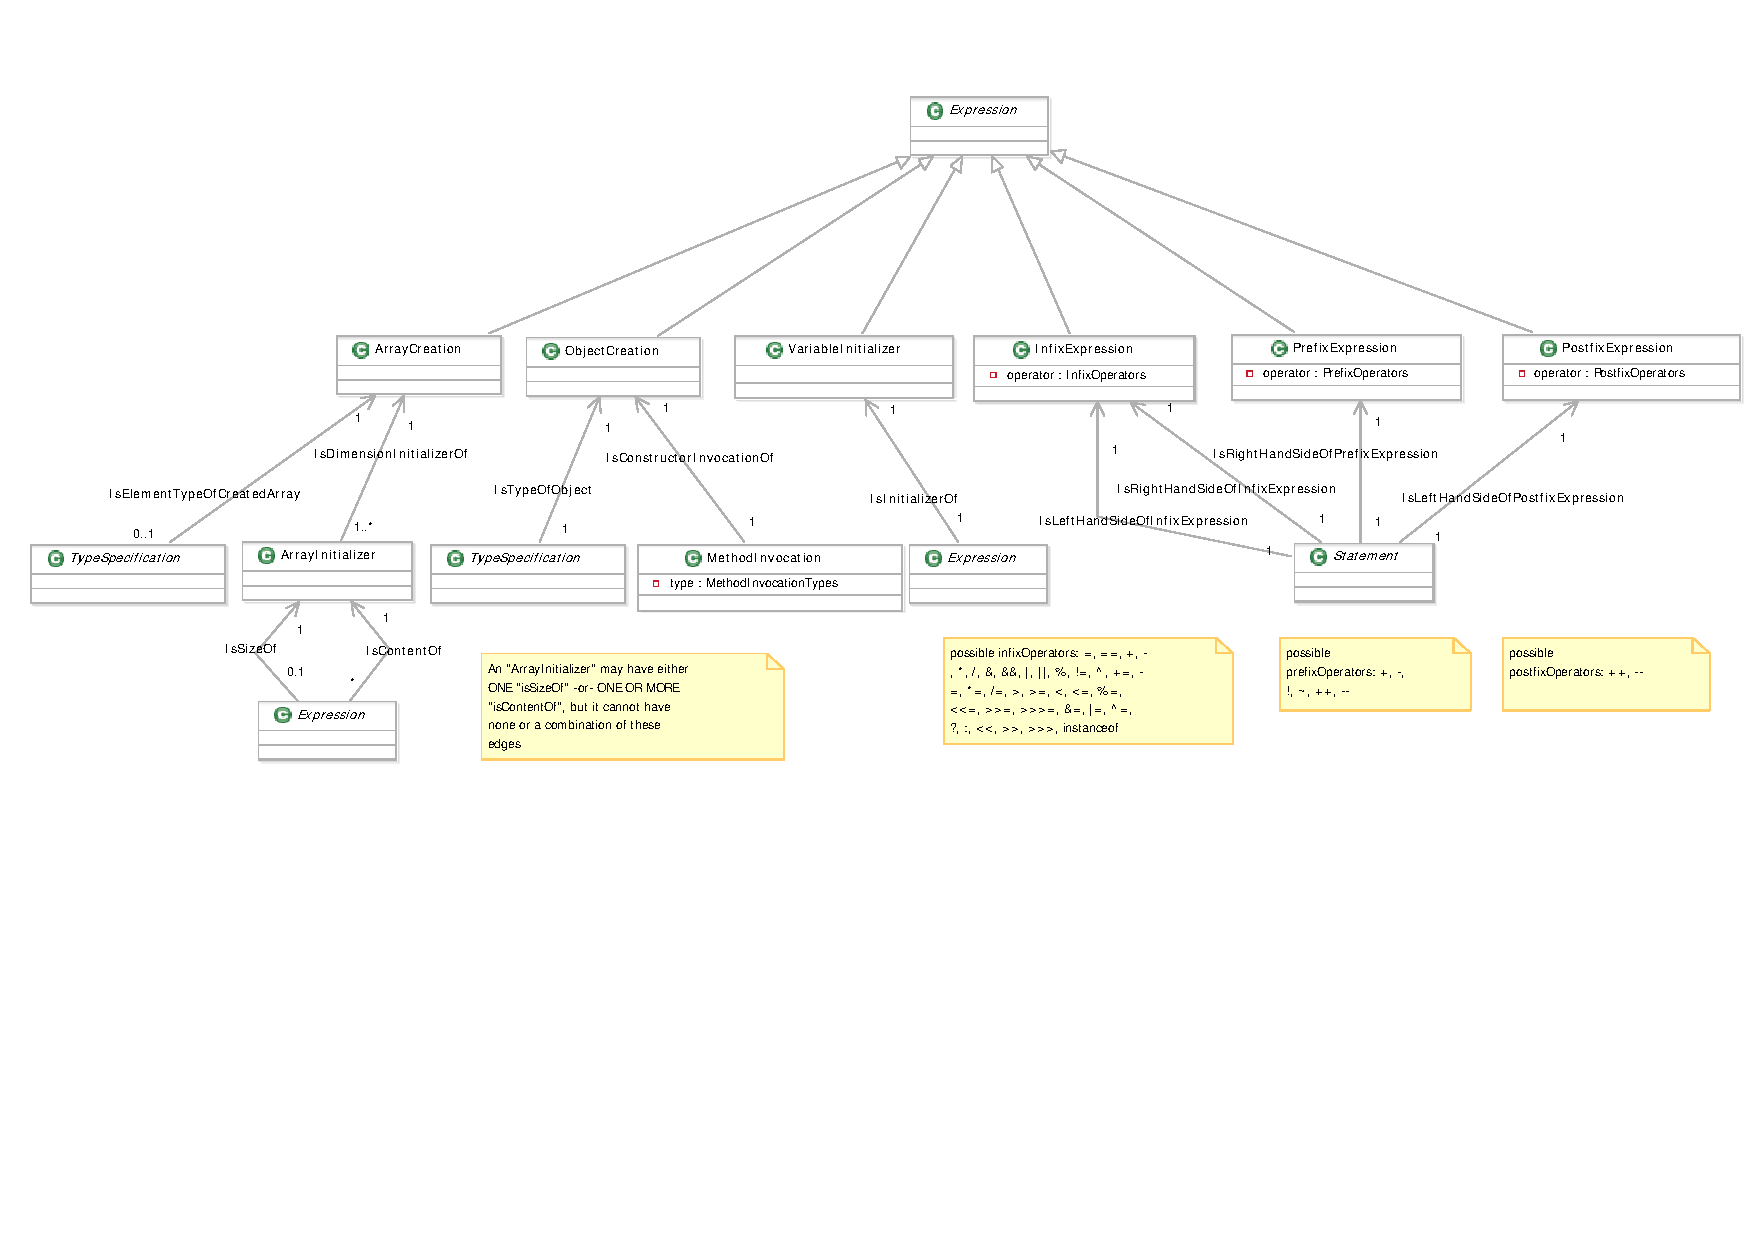
\includegraphics[width=19.8cm, angle=90]{figures/metamodell11.pdf}
	  \caption{Metamodell (Teil 11 / 12)}
  \end{center}
\end{figure}
\begin{figure}[htbp]
  \begin{center}
	  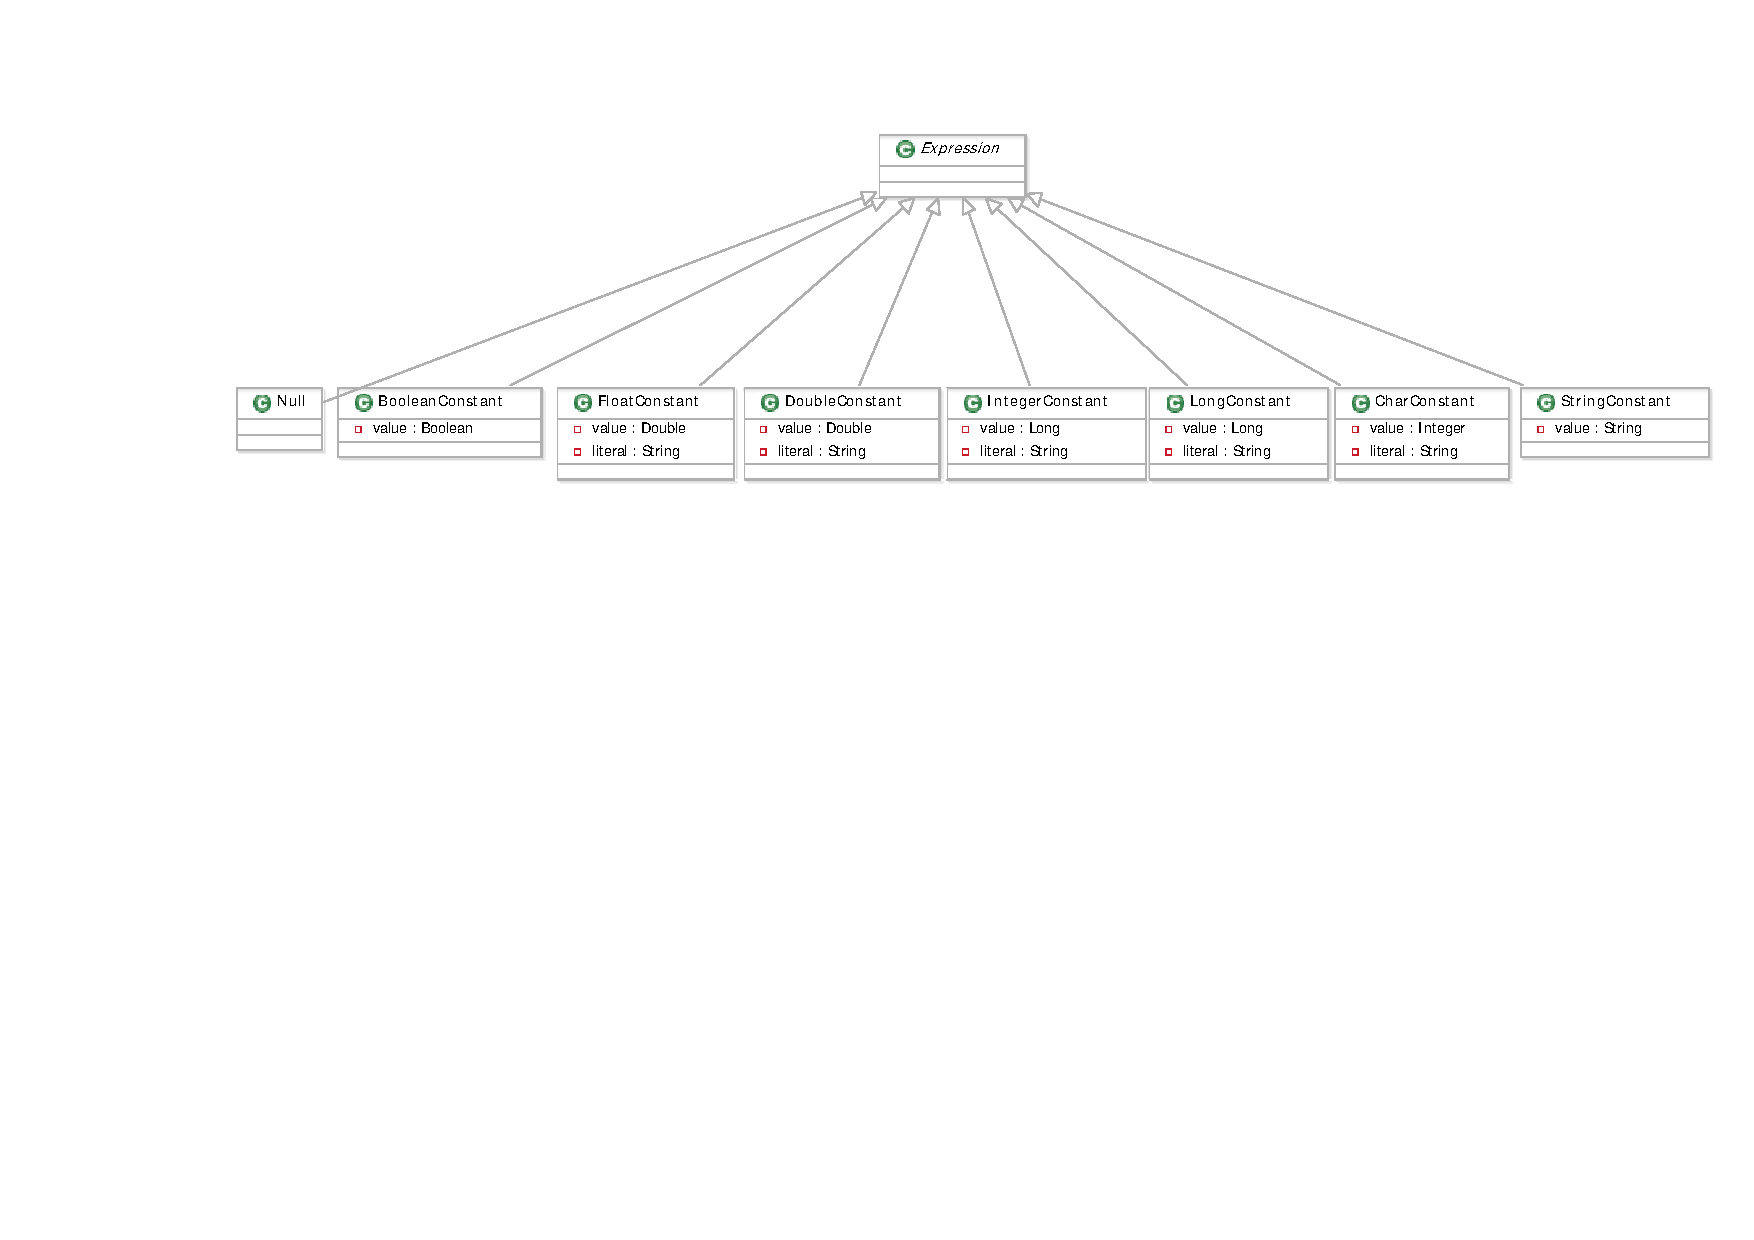
\includegraphics[width=19.8cm, angle=90]{figures/metamodell12.pdf}
	  \caption{Metamodell (Teil 12 / 12)}
  \end{center}
\end{figure}
\clearpage
\begin{figure}[htbp]
  \begin{center}
	  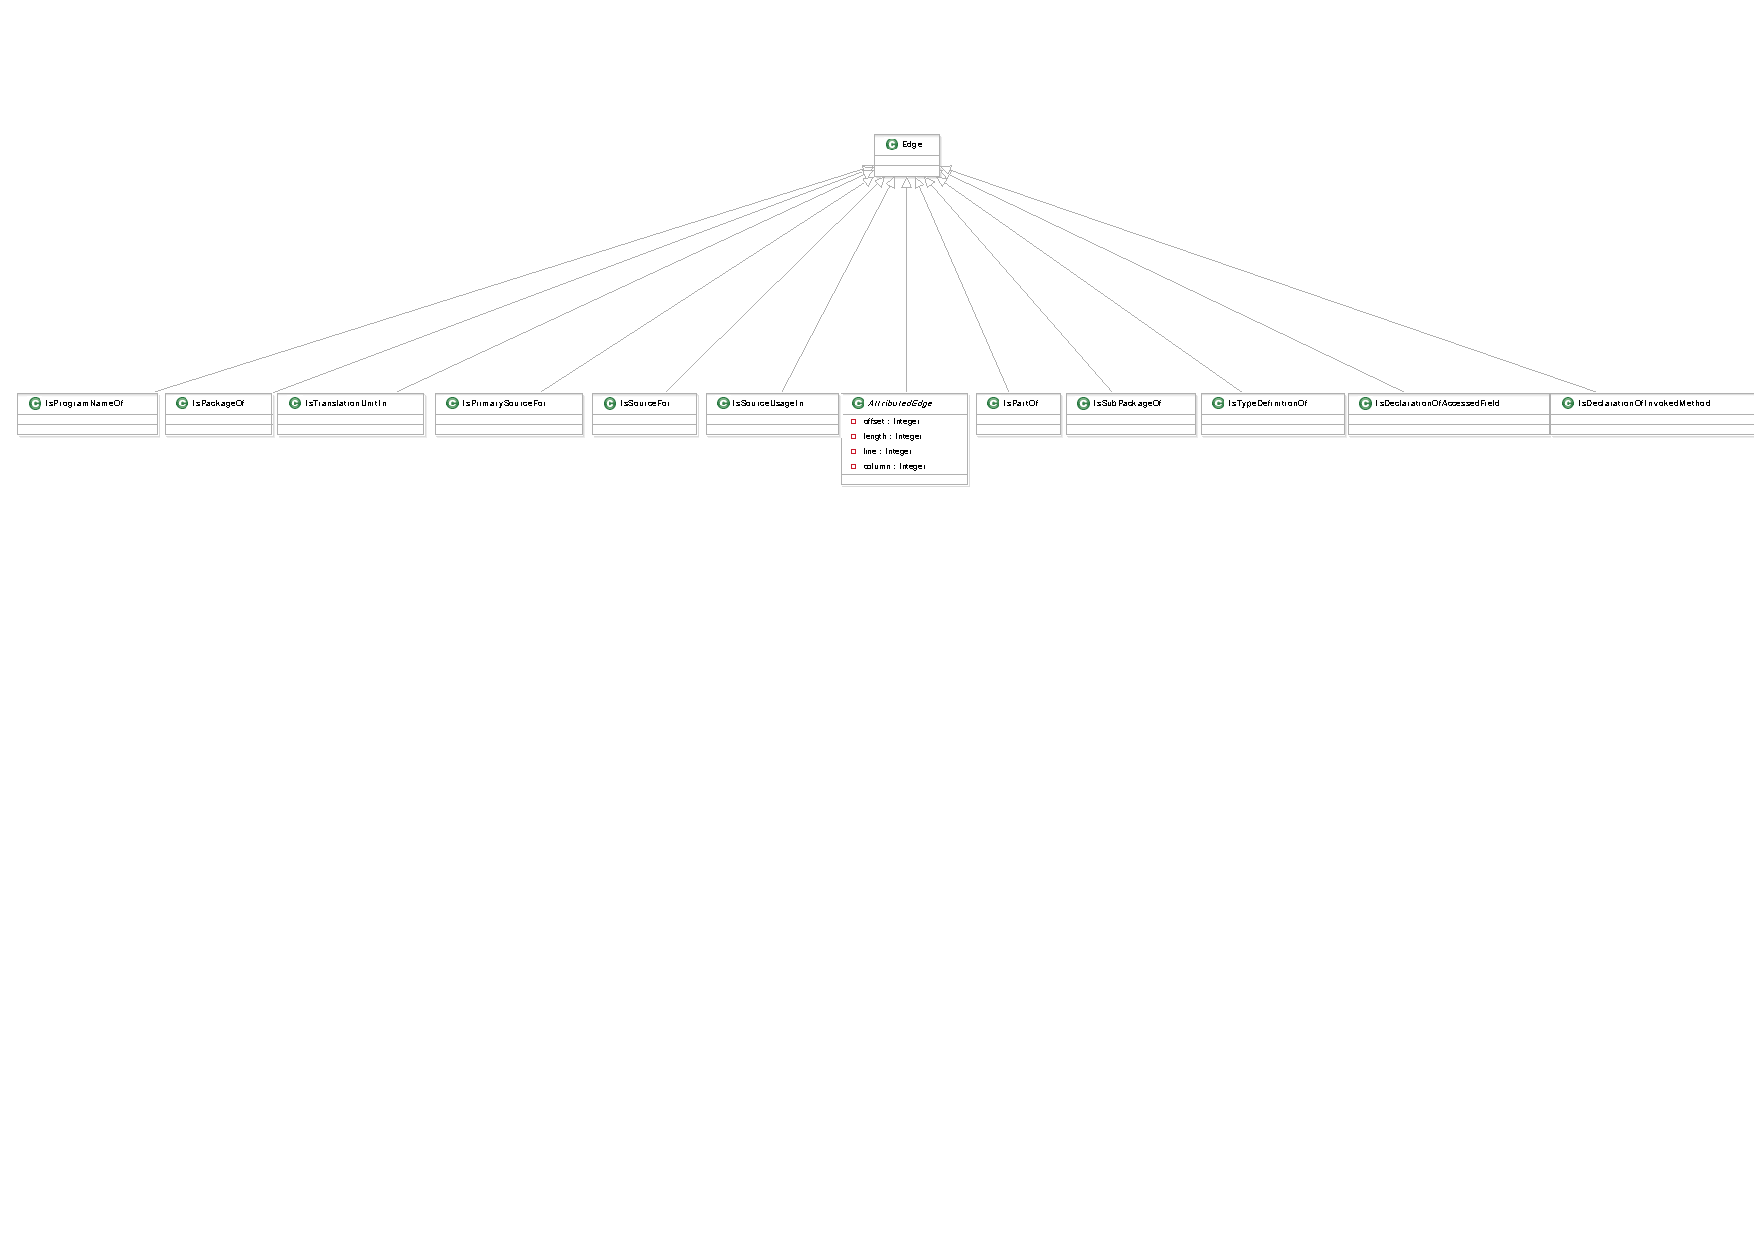
\includegraphics[width=19.8cm, angle=90]{figures/metamodellkanten01.pdf}
	  \caption{Kantentypenhierarchie (Teil 1 / 13)}
  \end{center}
\end{figure}
\begin{figure}[htbp]
  \begin{center}
	  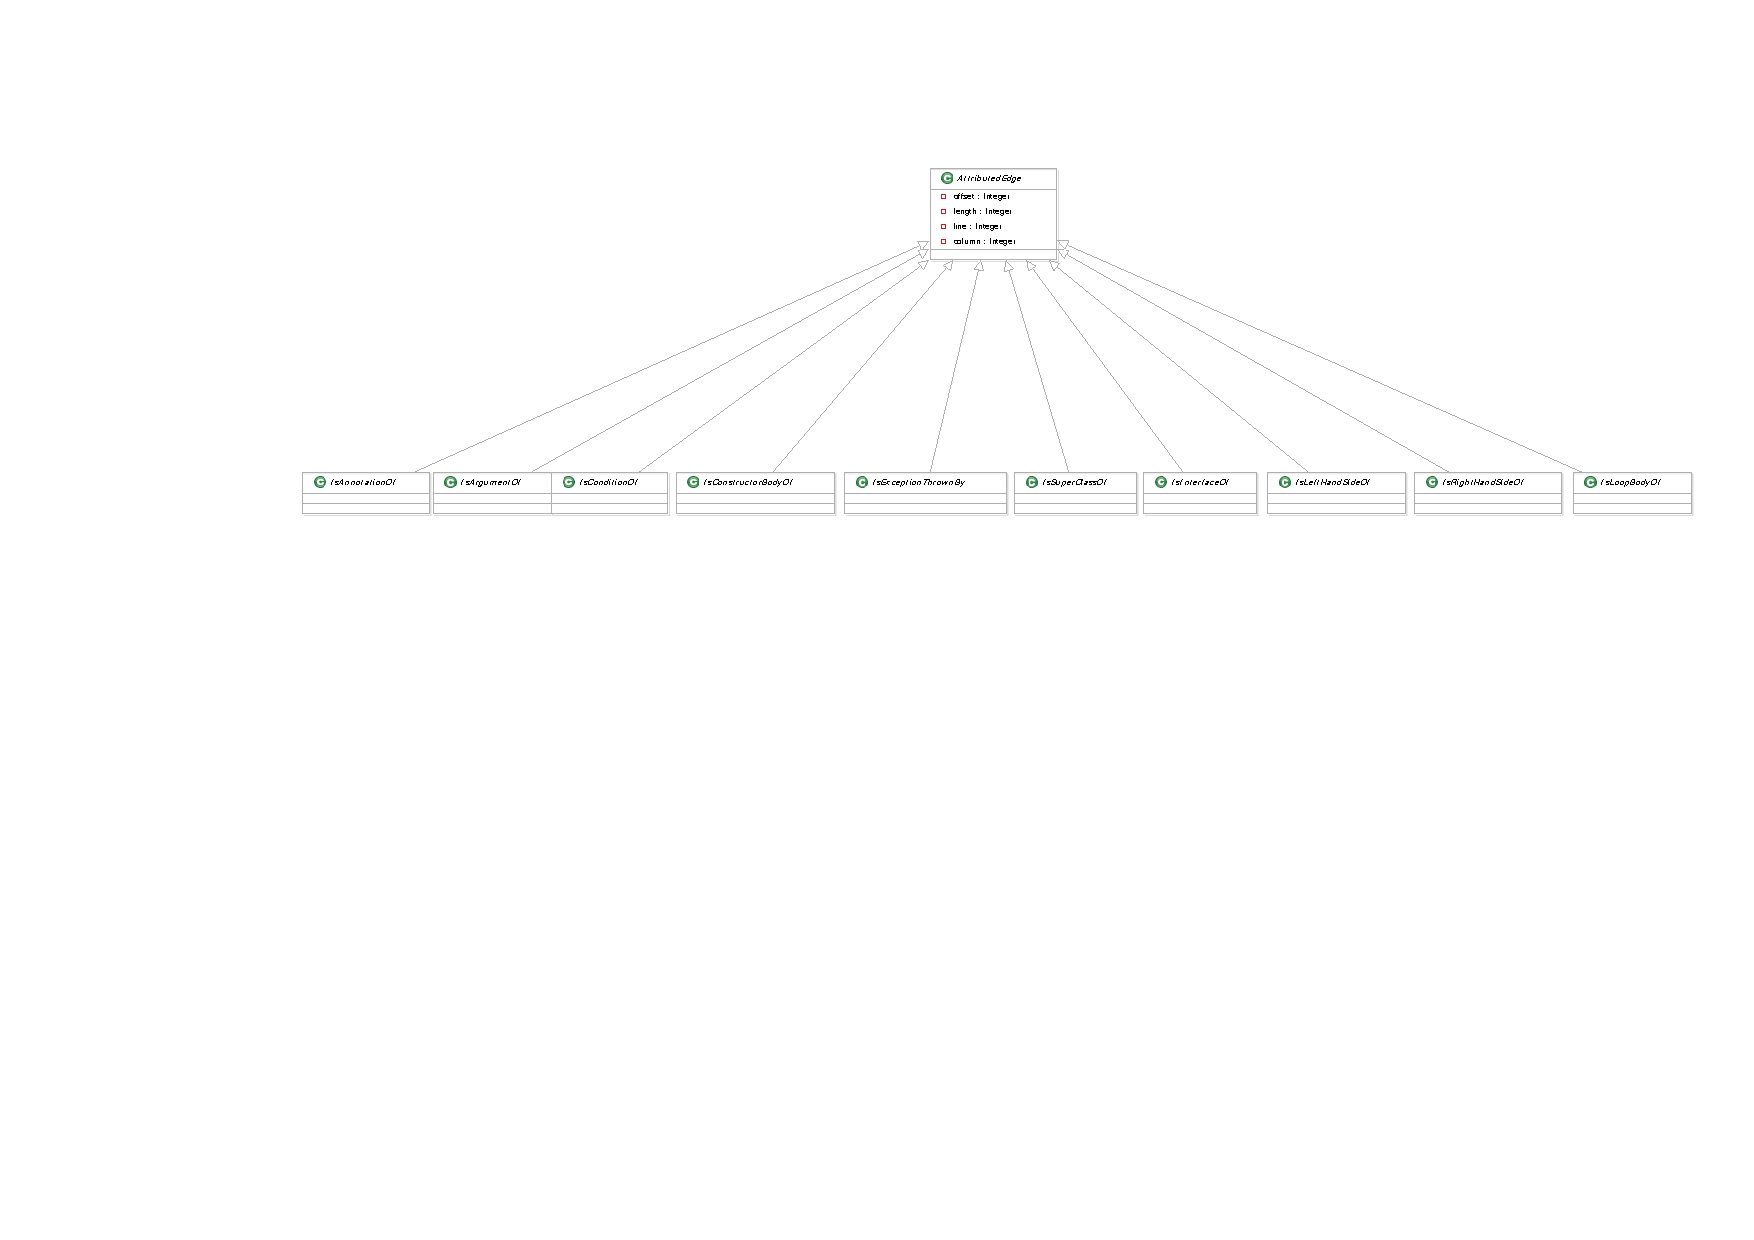
\includegraphics[width=19.8cm, angle=90]{figures/metamodellkanten02.pdf}
	  \caption{Kantentypenhierarchie (Teil 2 / 13)}
  \end{center}
\end{figure}
\begin{figure}[htbp]
  \begin{center}
	  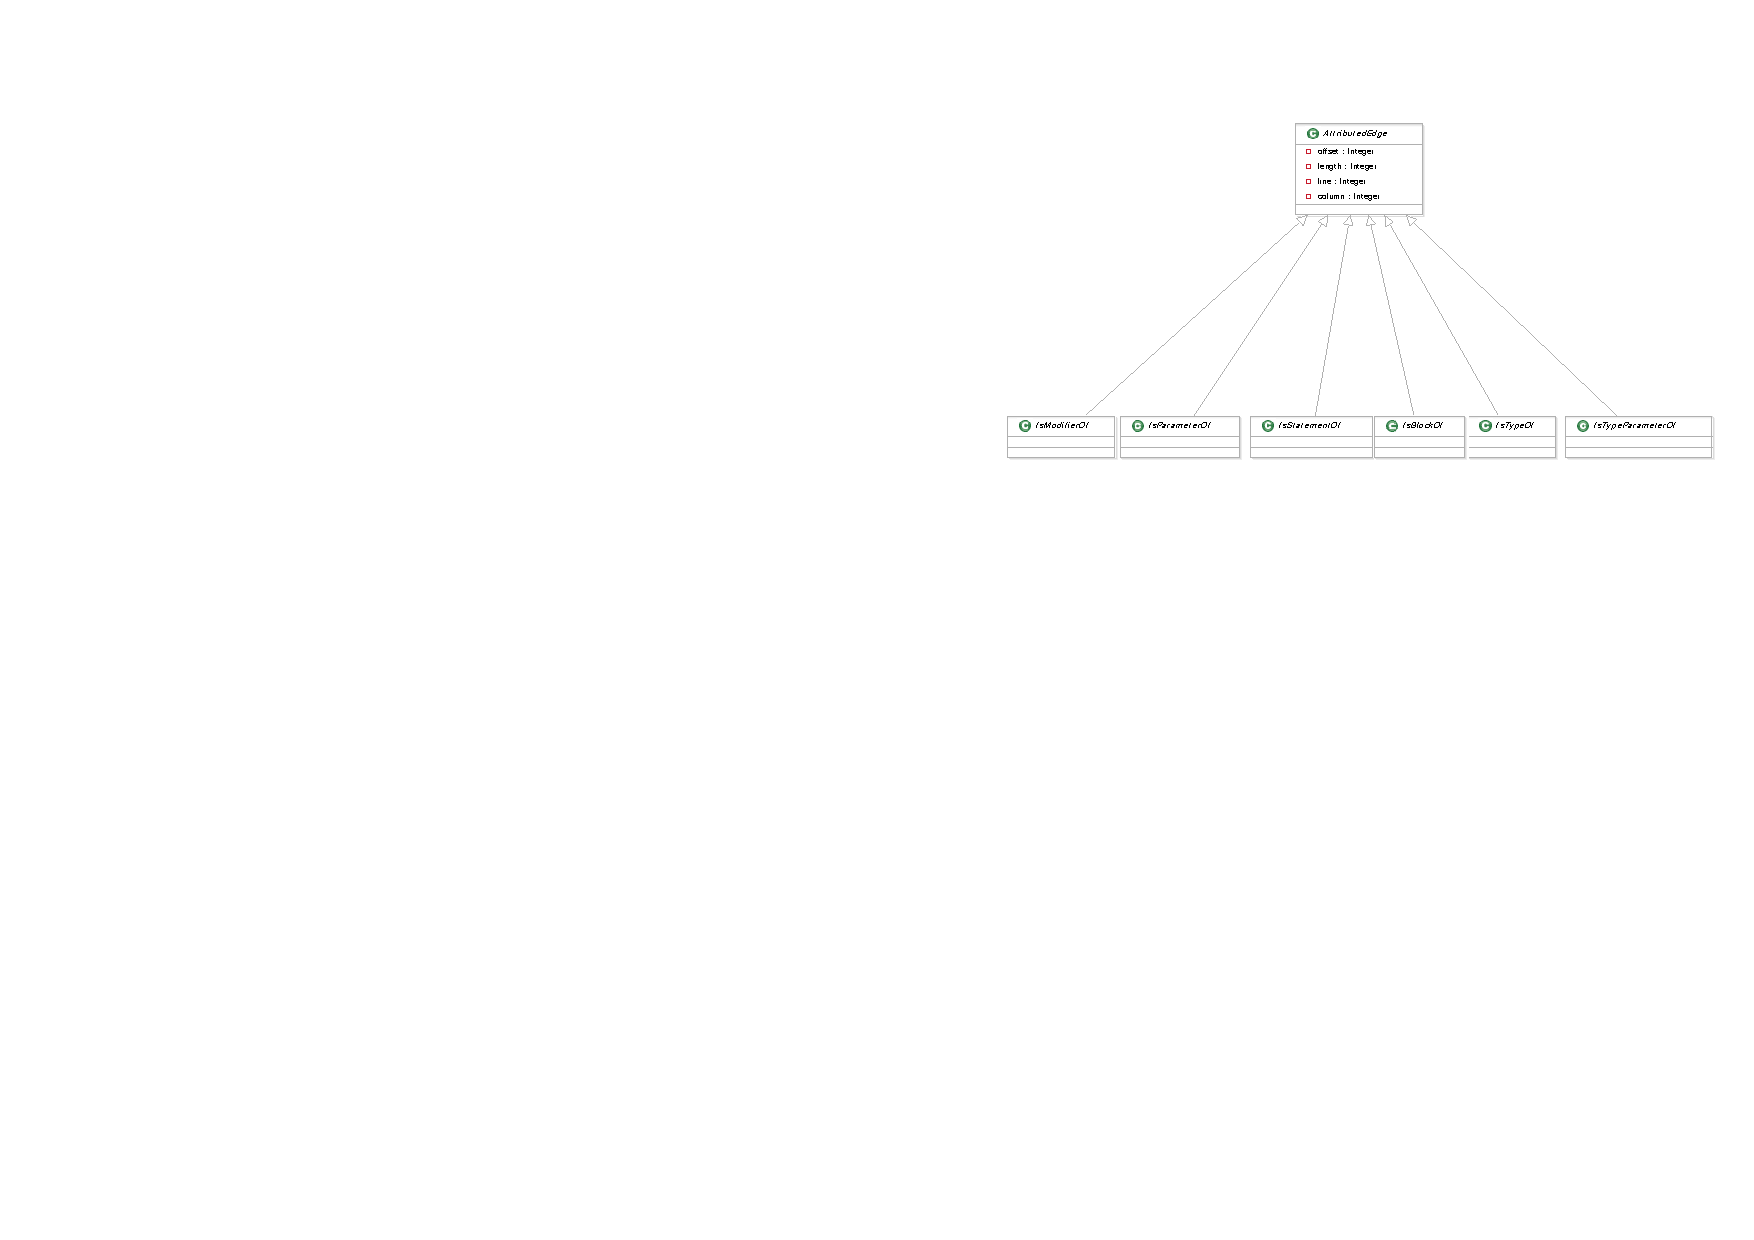
\includegraphics[width=19.8cm, angle=90]{figures/metamodellkanten03.pdf}
	  \caption{Kantentypenhierarchie (Teil 3 / 13)}
  \end{center}
\end{figure}
\begin{figure}[htbp]
  \begin{center}
	  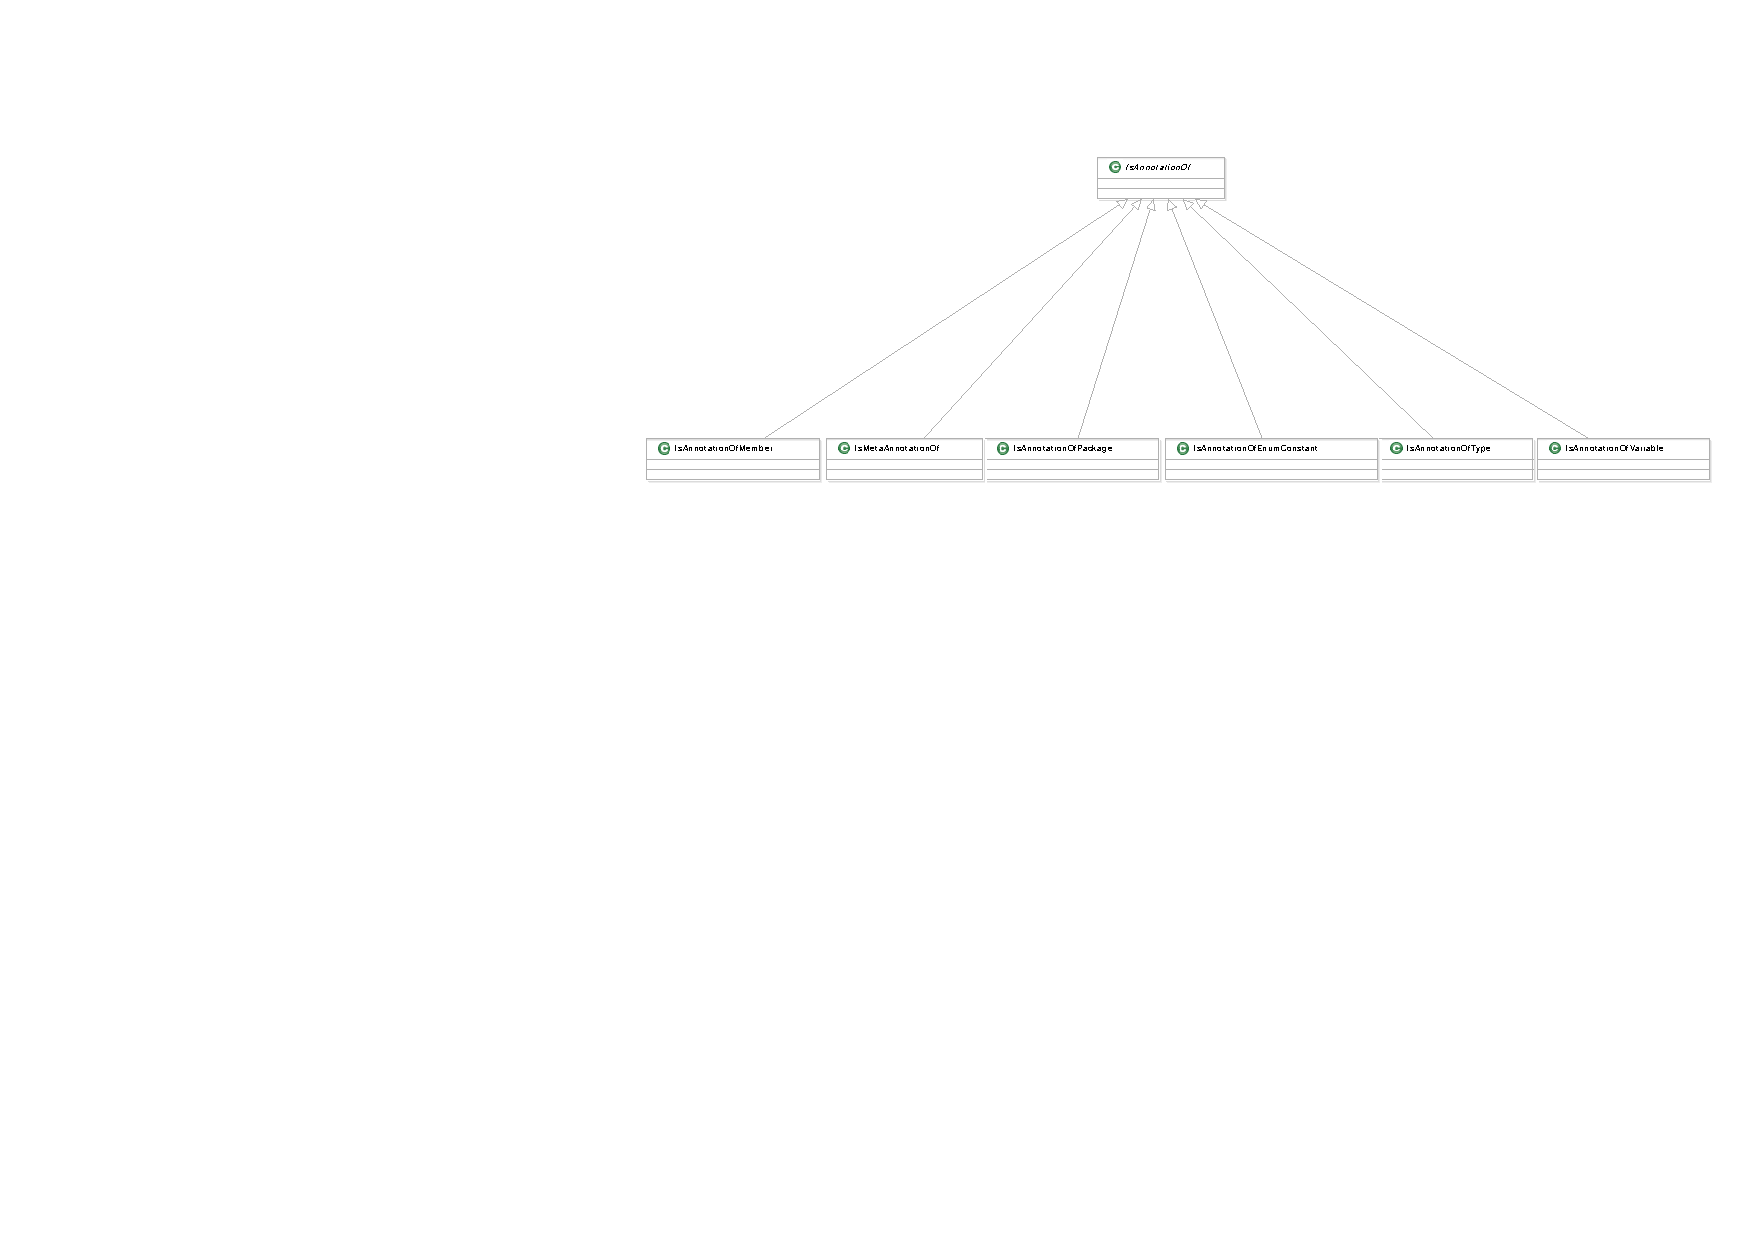
\includegraphics[width=19.8cm, angle=90]{figures/metamodellkanten04.pdf}
	  \caption{Kantentypenhierarchie (Teil 4 / 13)}
  \end{center}
\end{figure}
\begin{figure}[htbp]
  \begin{center}
	  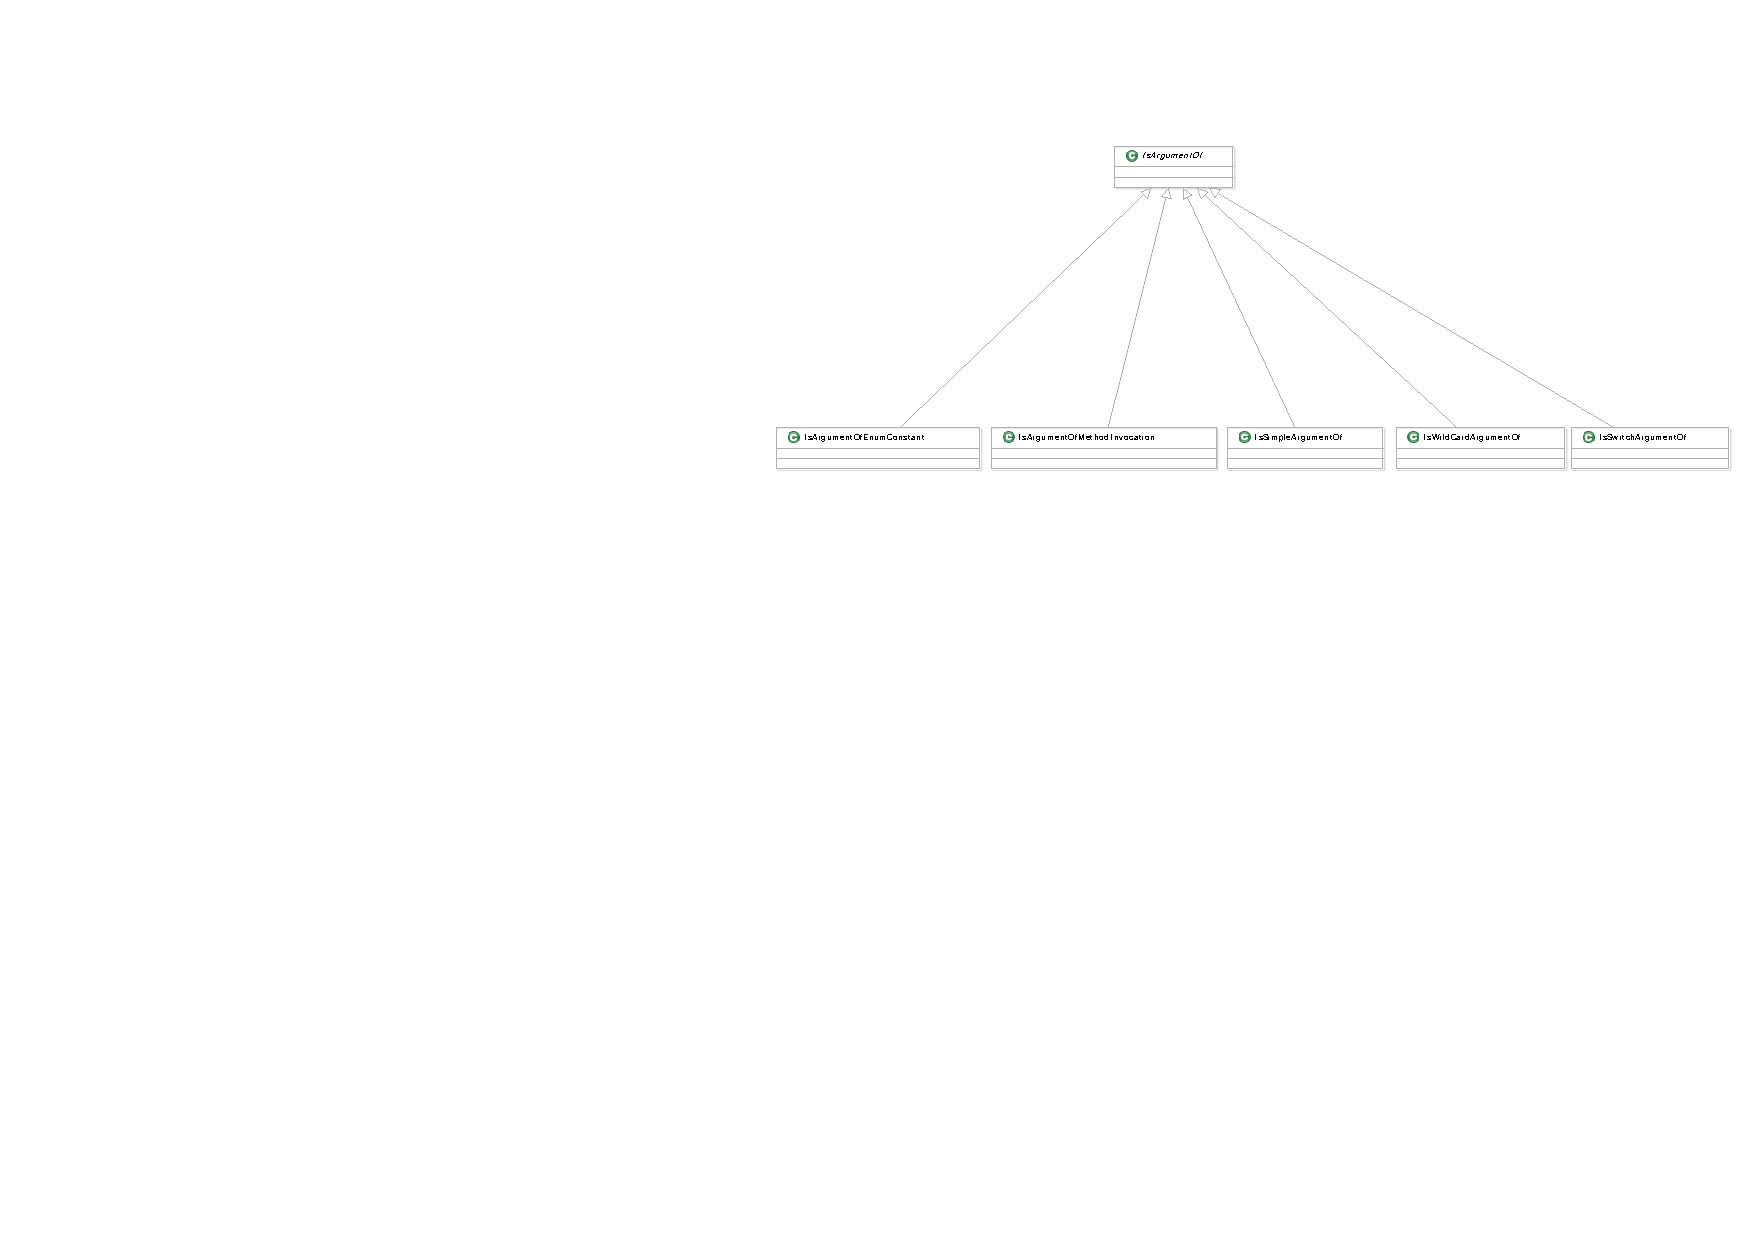
\includegraphics[width=19.8cm, angle=90]{figures/metamodellkanten05.pdf}
	  \caption{Kantentypenhierarchie (Teil 5 / 13)}
  \end{center}
\end{figure}
\begin{figure}[htbp]
  \begin{center}
	  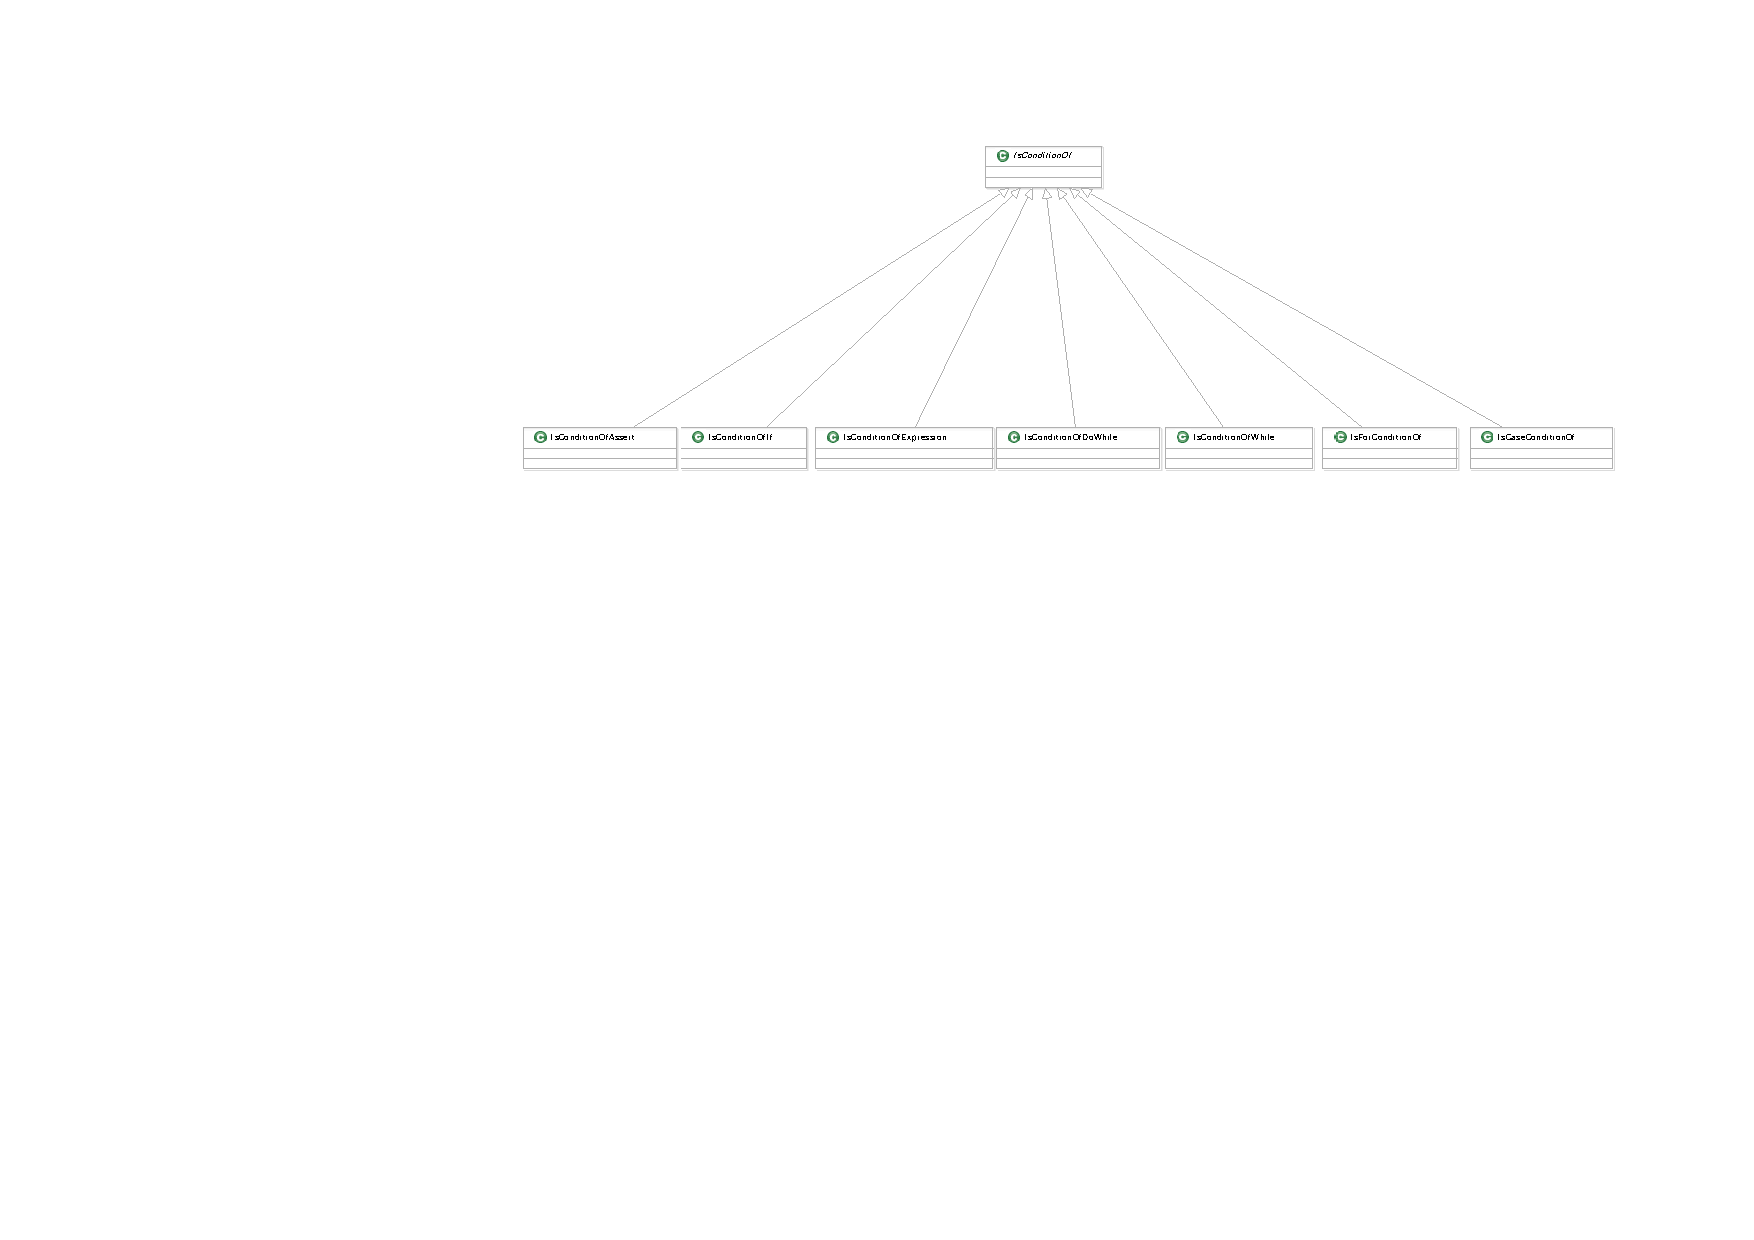
\includegraphics[width=19.8cm, angle=90]{figures/metamodellkanten06.pdf}
	  \caption{Kantentypenhierarchie (Teil 6 / 13)}
  \end{center}
\end{figure}
\begin{figure}[htbp]
  \begin{center}
	  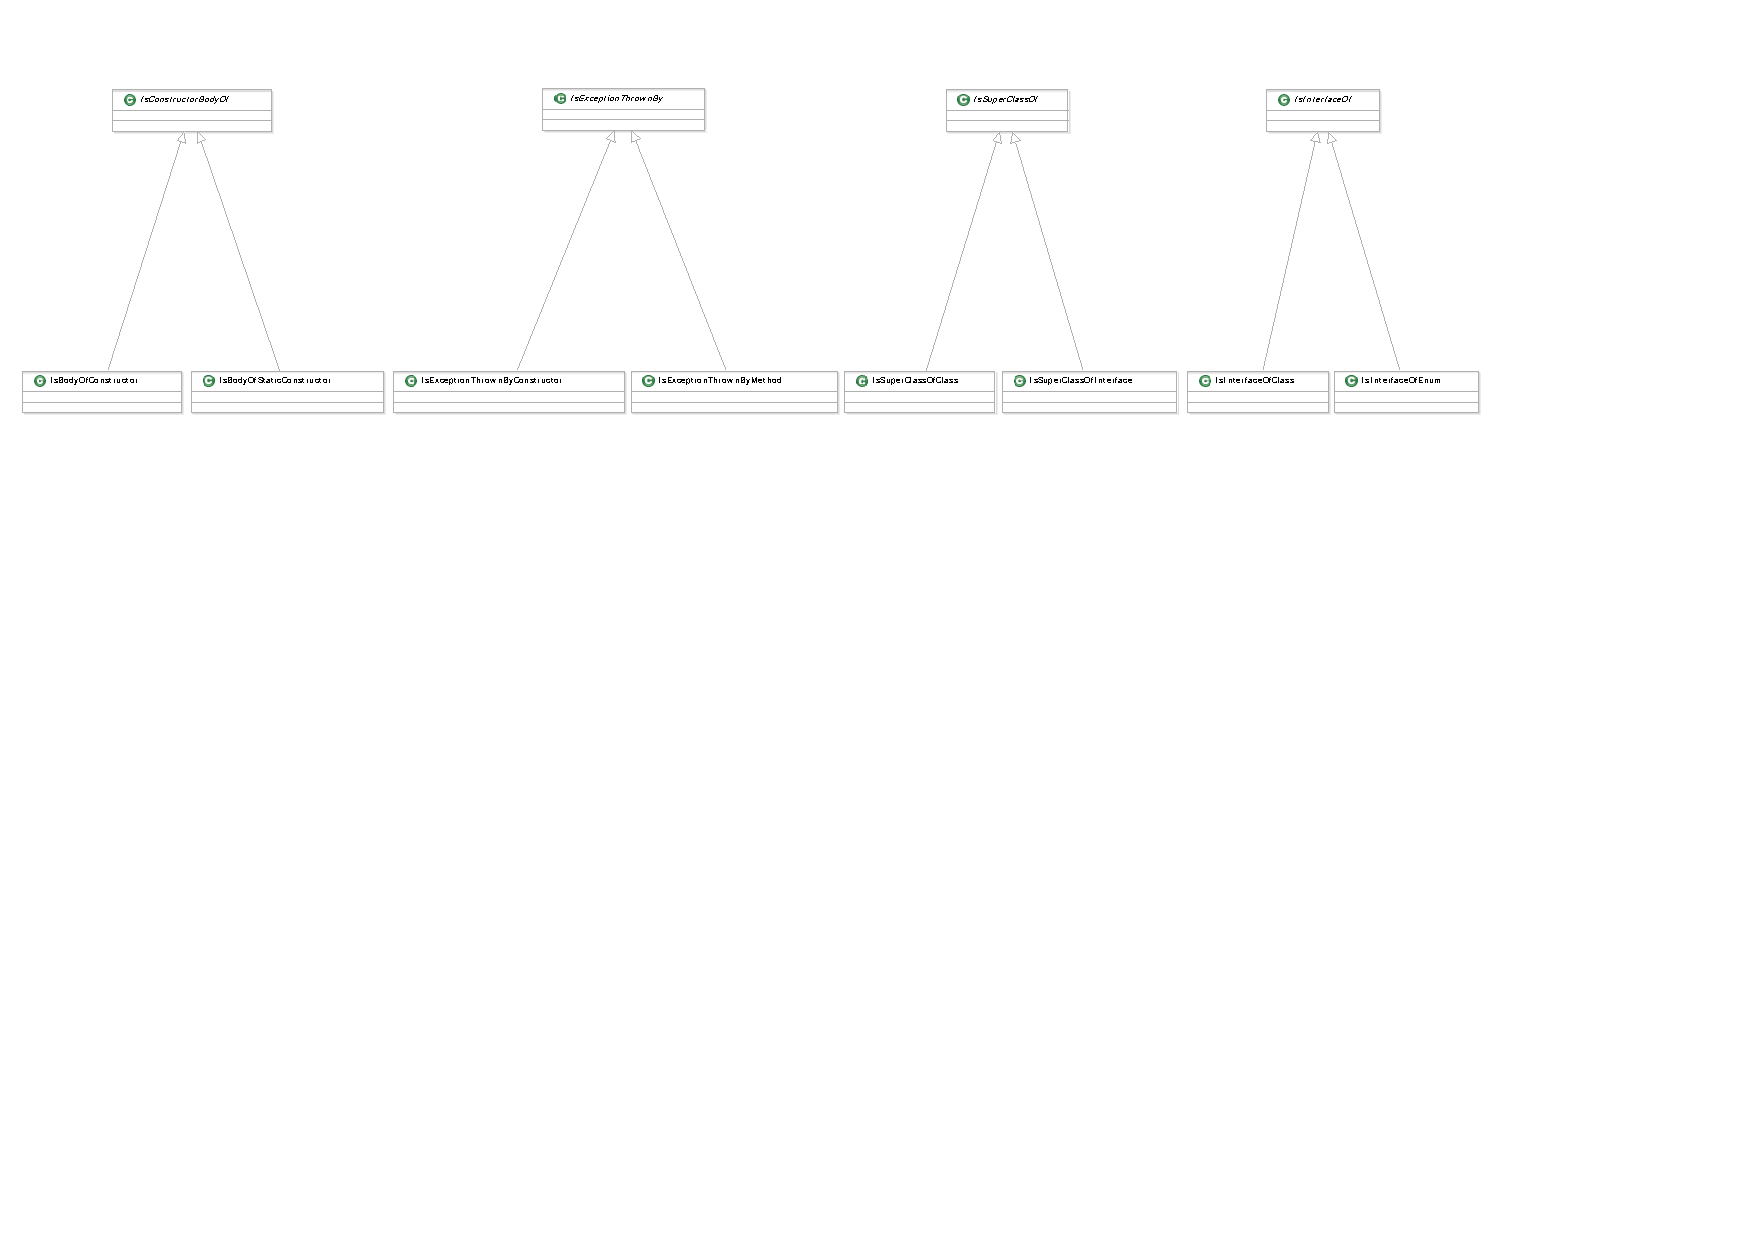
\includegraphics[width=19.8cm, angle=90]{figures/metamodellkanten07.pdf}
	  \caption{Kantentypenhierarchie (Teil 7 / 13)}
  \end{center}
\end{figure}
\begin{figure}[htbp]
  \begin{center}
	  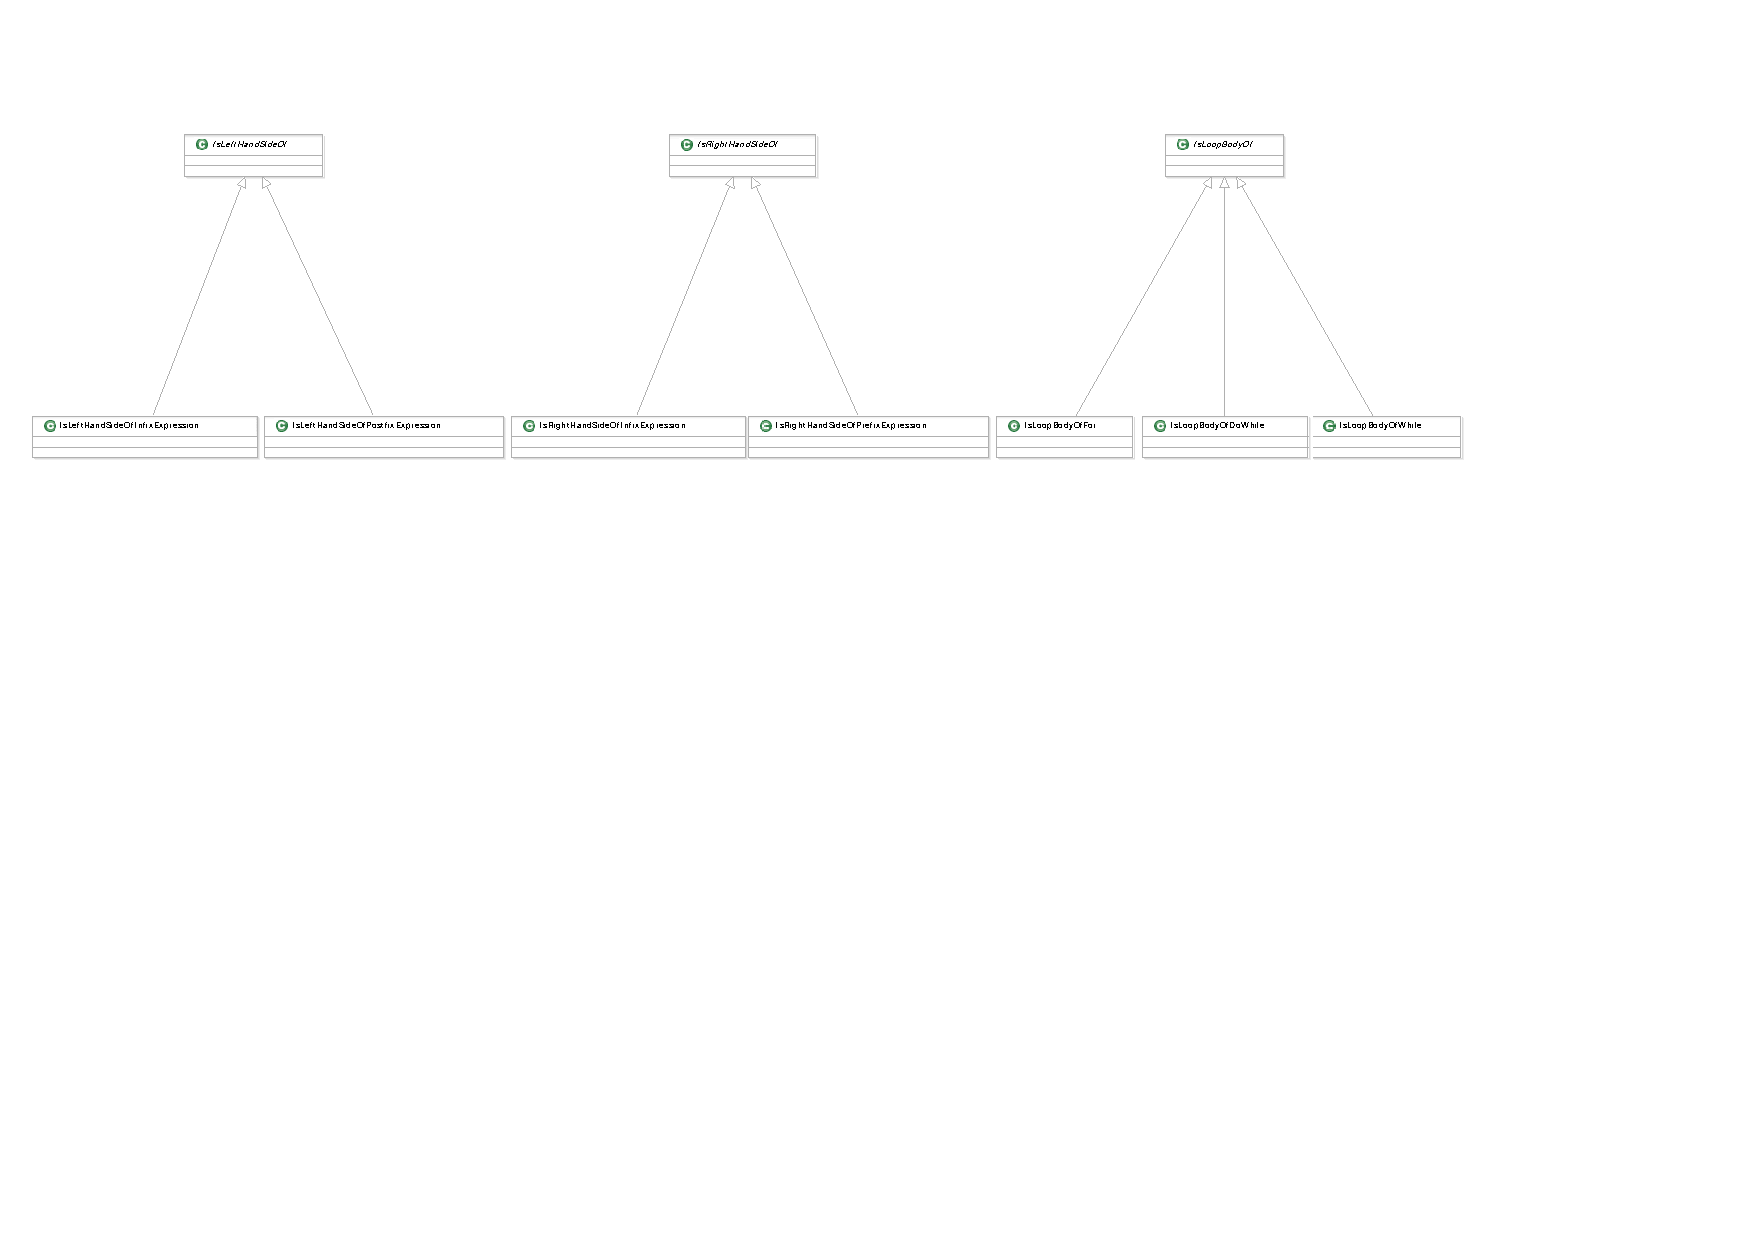
\includegraphics[width=19.8cm, angle=90]{figures/metamodellkanten08.pdf}
	  \caption{Kantentypenhierarchie (Teil 8 / 13)}
  \end{center}
\end{figure}
\begin{figure}[htbp]
  \begin{center}
	  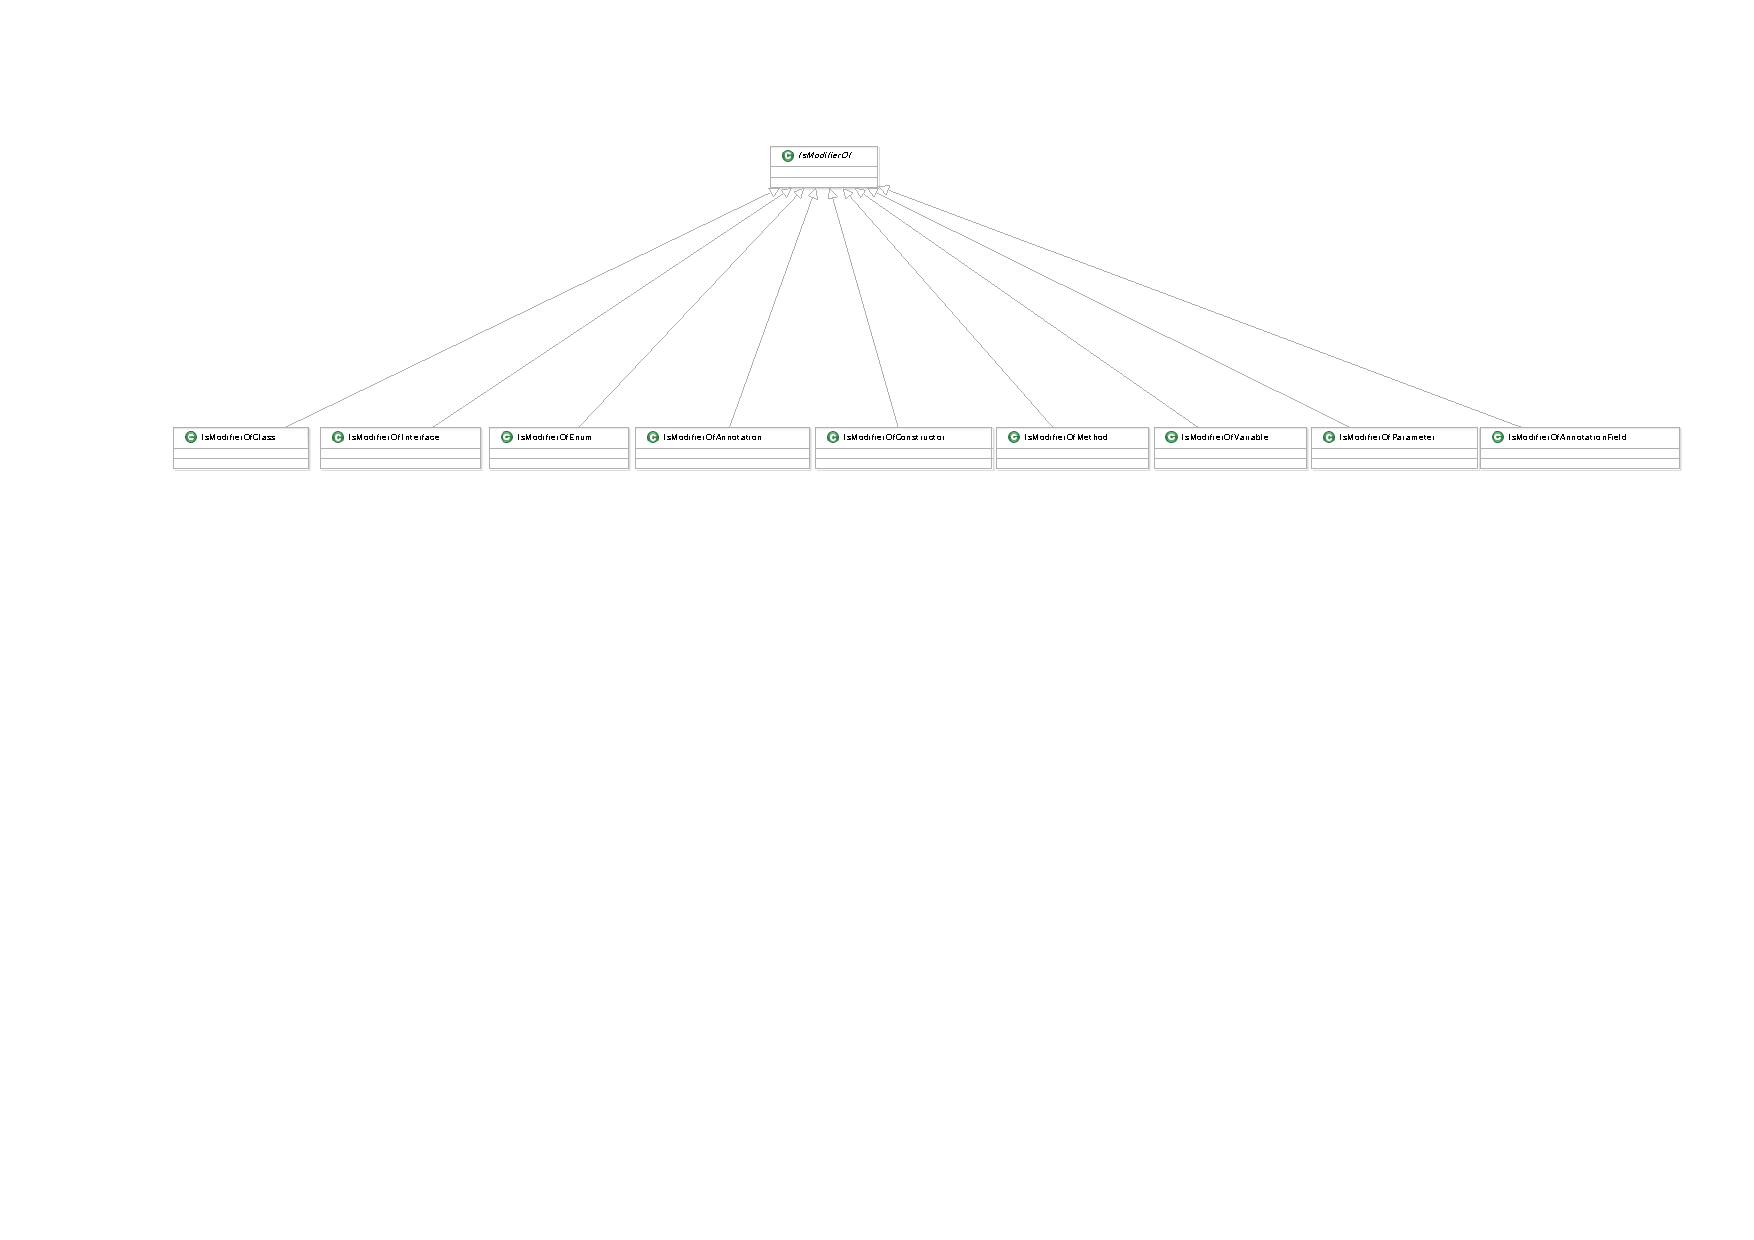
\includegraphics[width=19.8cm, angle=90]{figures/metamodellkanten09.pdf}
	  \caption{Kantentypenhierarchie (Teil 9 / 13)}
  \end{center}
\end{figure}
\begin{figure}[htbp]
  \begin{center}
	  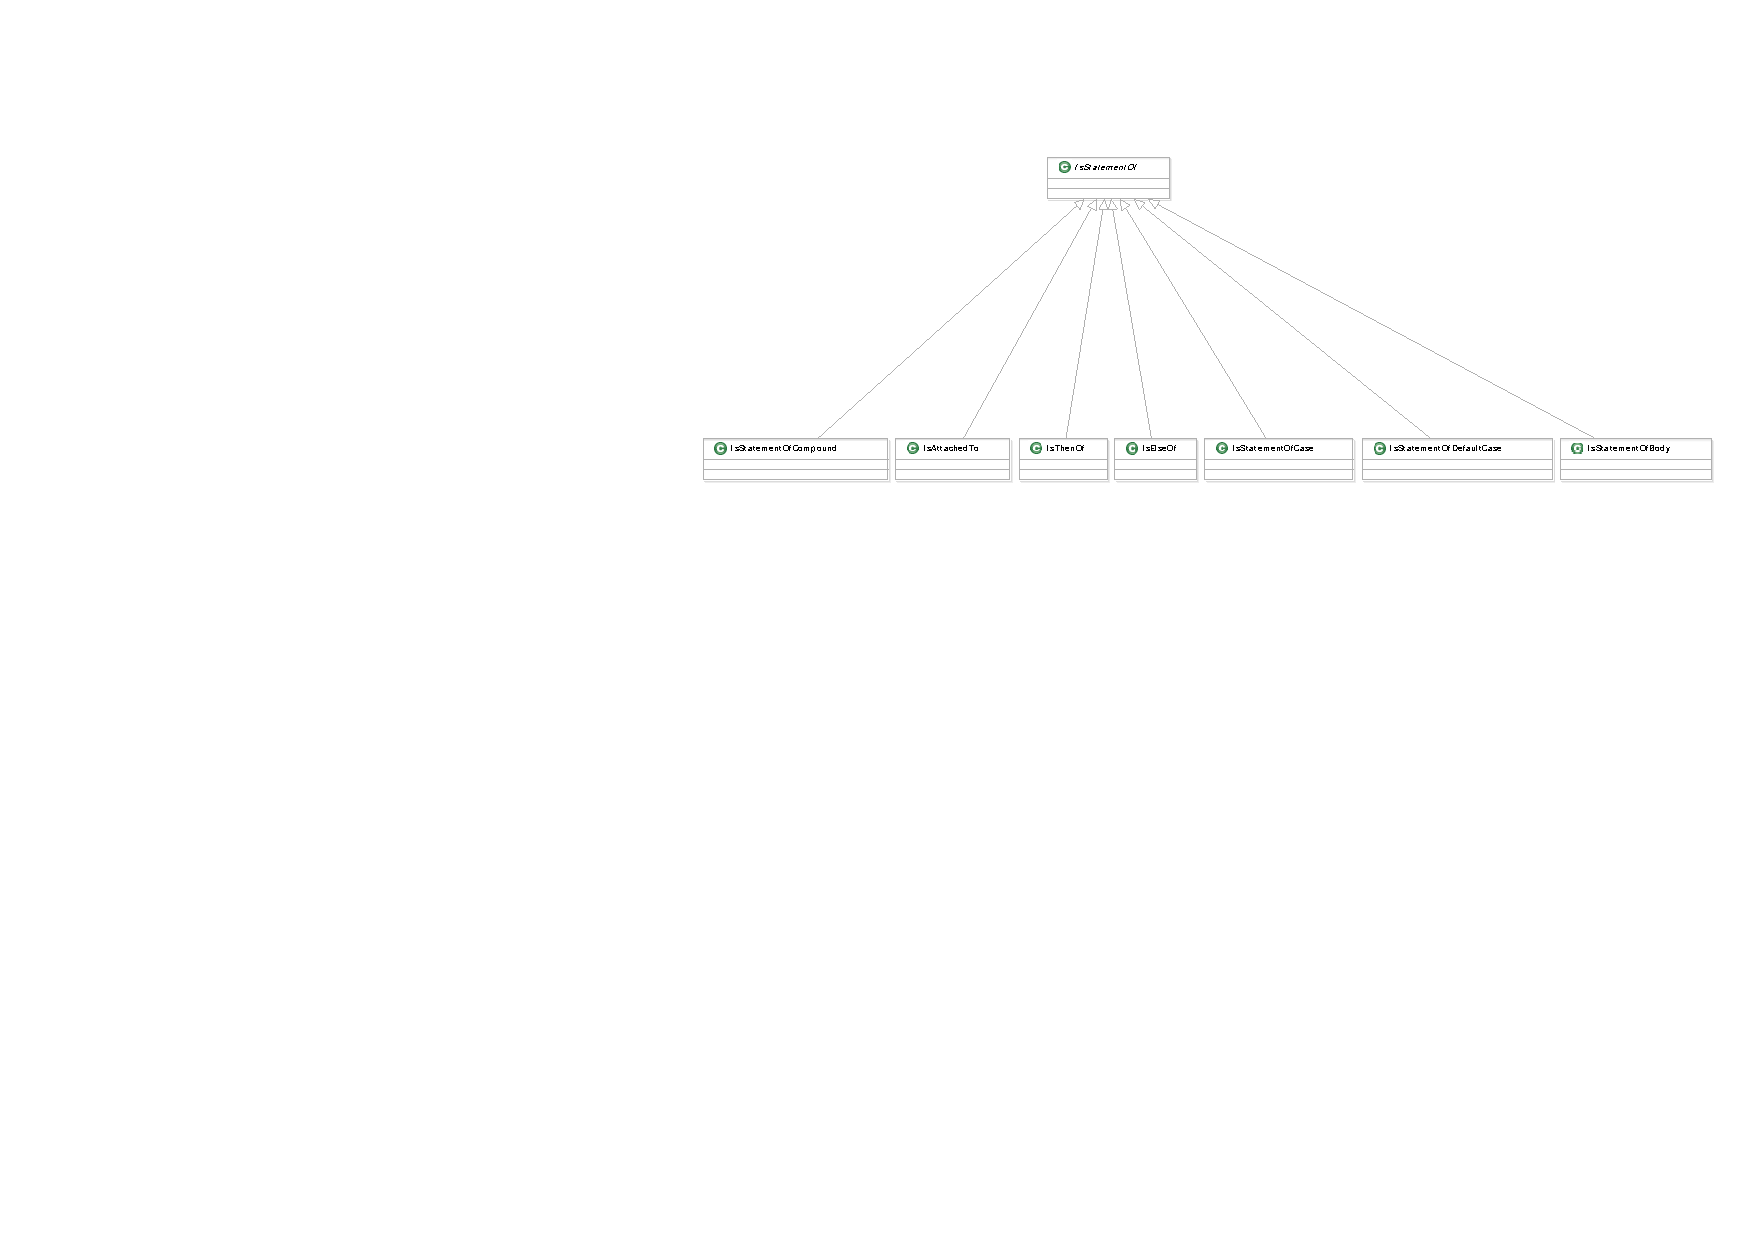
\includegraphics[width=19.8cm, angle=90]{figures/metamodellkanten10.pdf}
	  \caption{Kantentypenhierarchie (Teil 10 / 13)}
  \end{center}
\end{figure}
\begin{figure}[htbp]
  \begin{center}
	  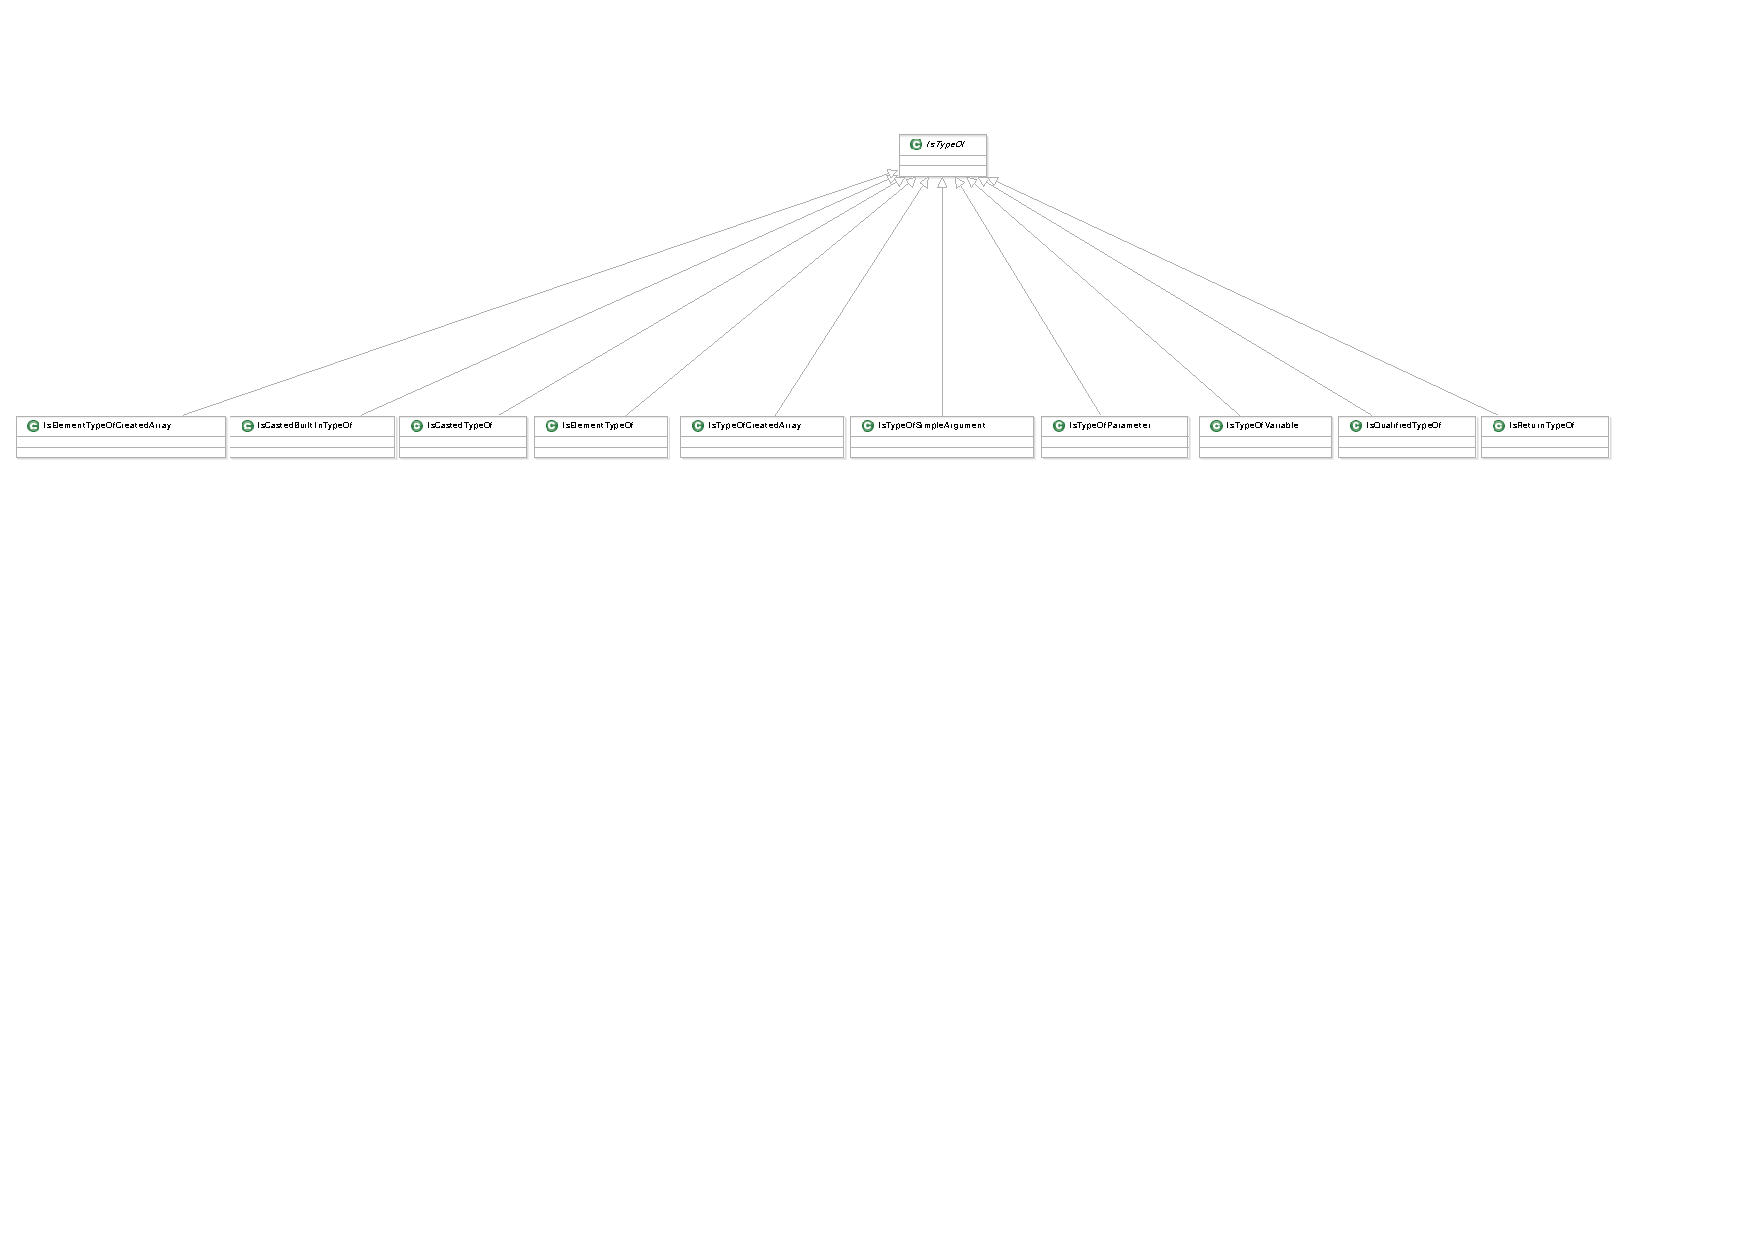
\includegraphics[width=19.8cm, angle=90]{figures/metamodellkanten11.pdf}
	  \caption{Kantentypenhierarchie (Teil 11 / 13)}
  \end{center}
\end{figure}
\begin{figure}[htbp]
  \begin{center}
	  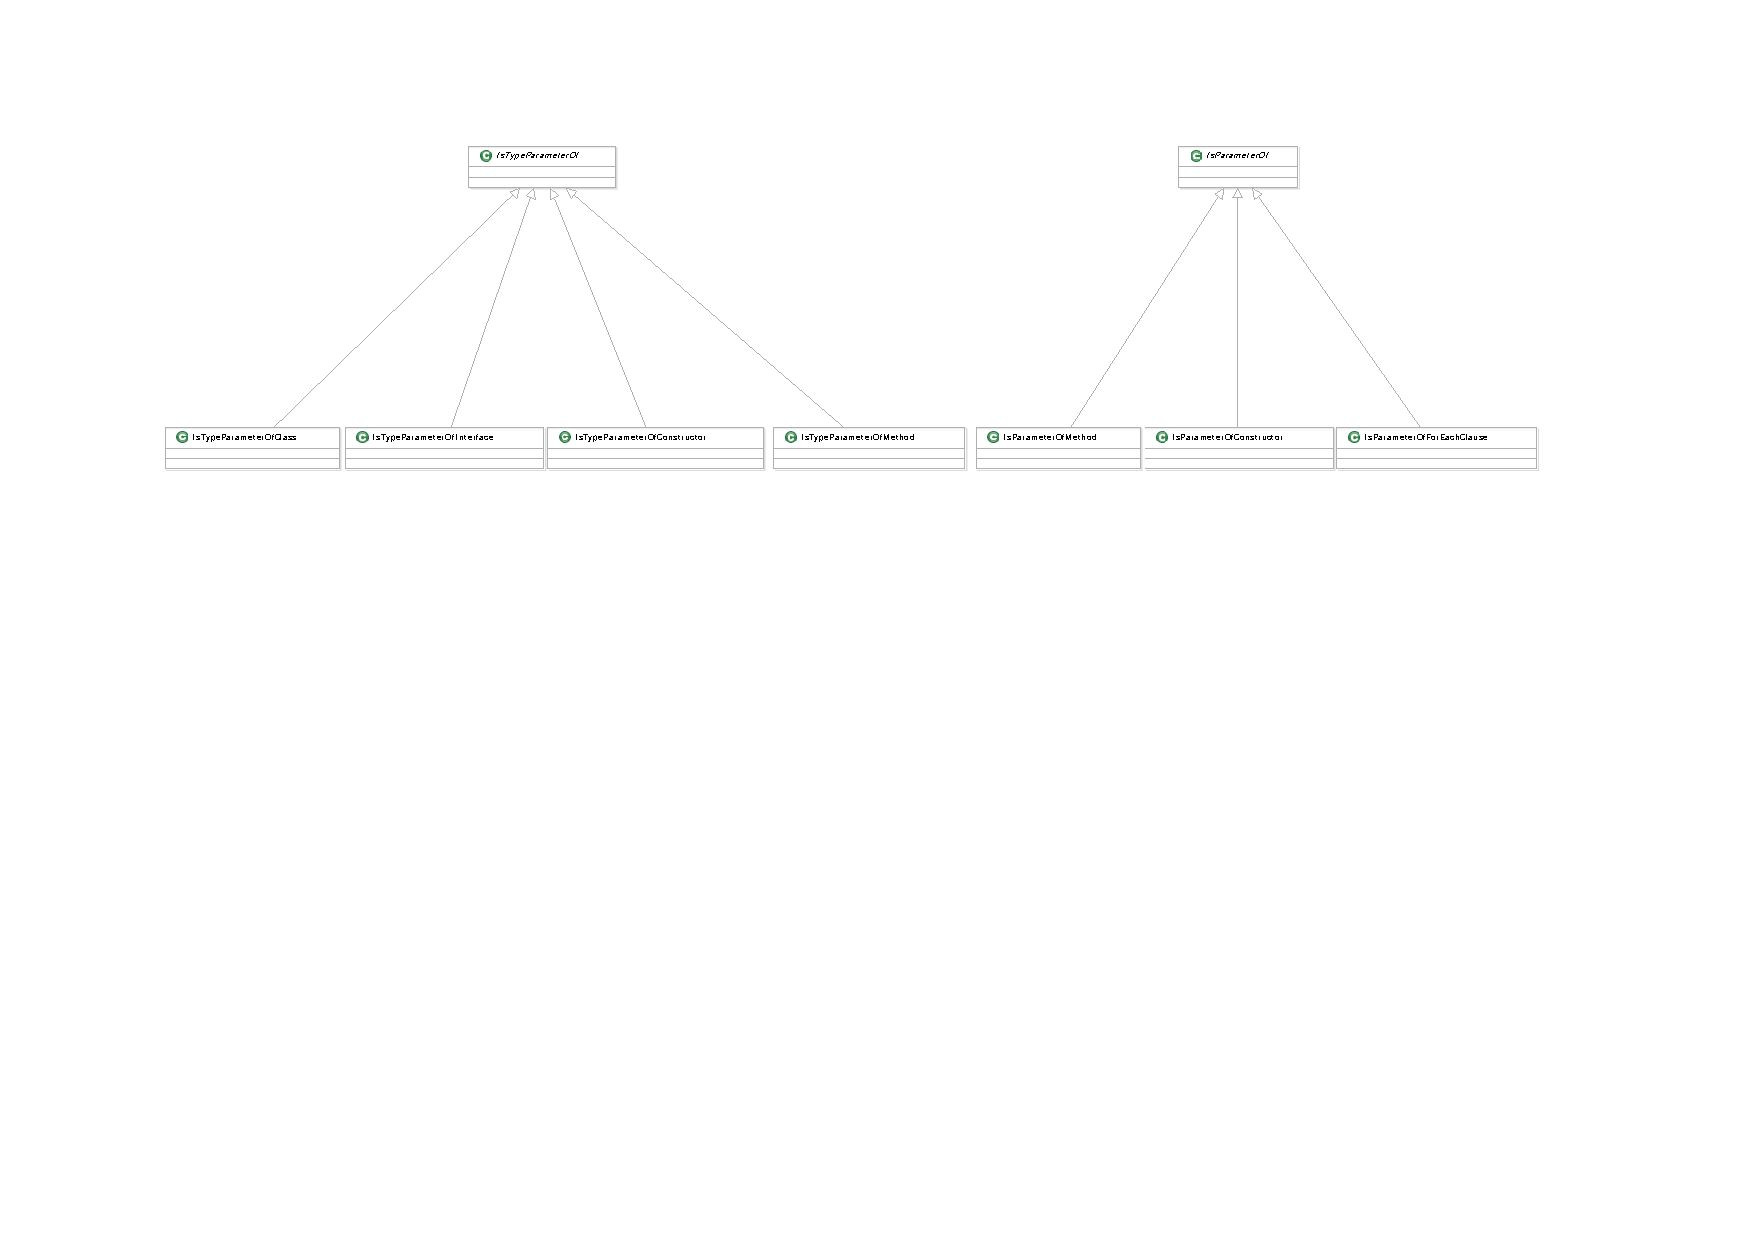
\includegraphics[width=19.8cm, angle=90]{figures/metamodellkanten12.pdf}
	  \caption{Kantentypenhierarchie (Teil 12 / 13)}
  \end{center}
\end{figure}
\begin{figure}[htbp]
  \begin{center}
	  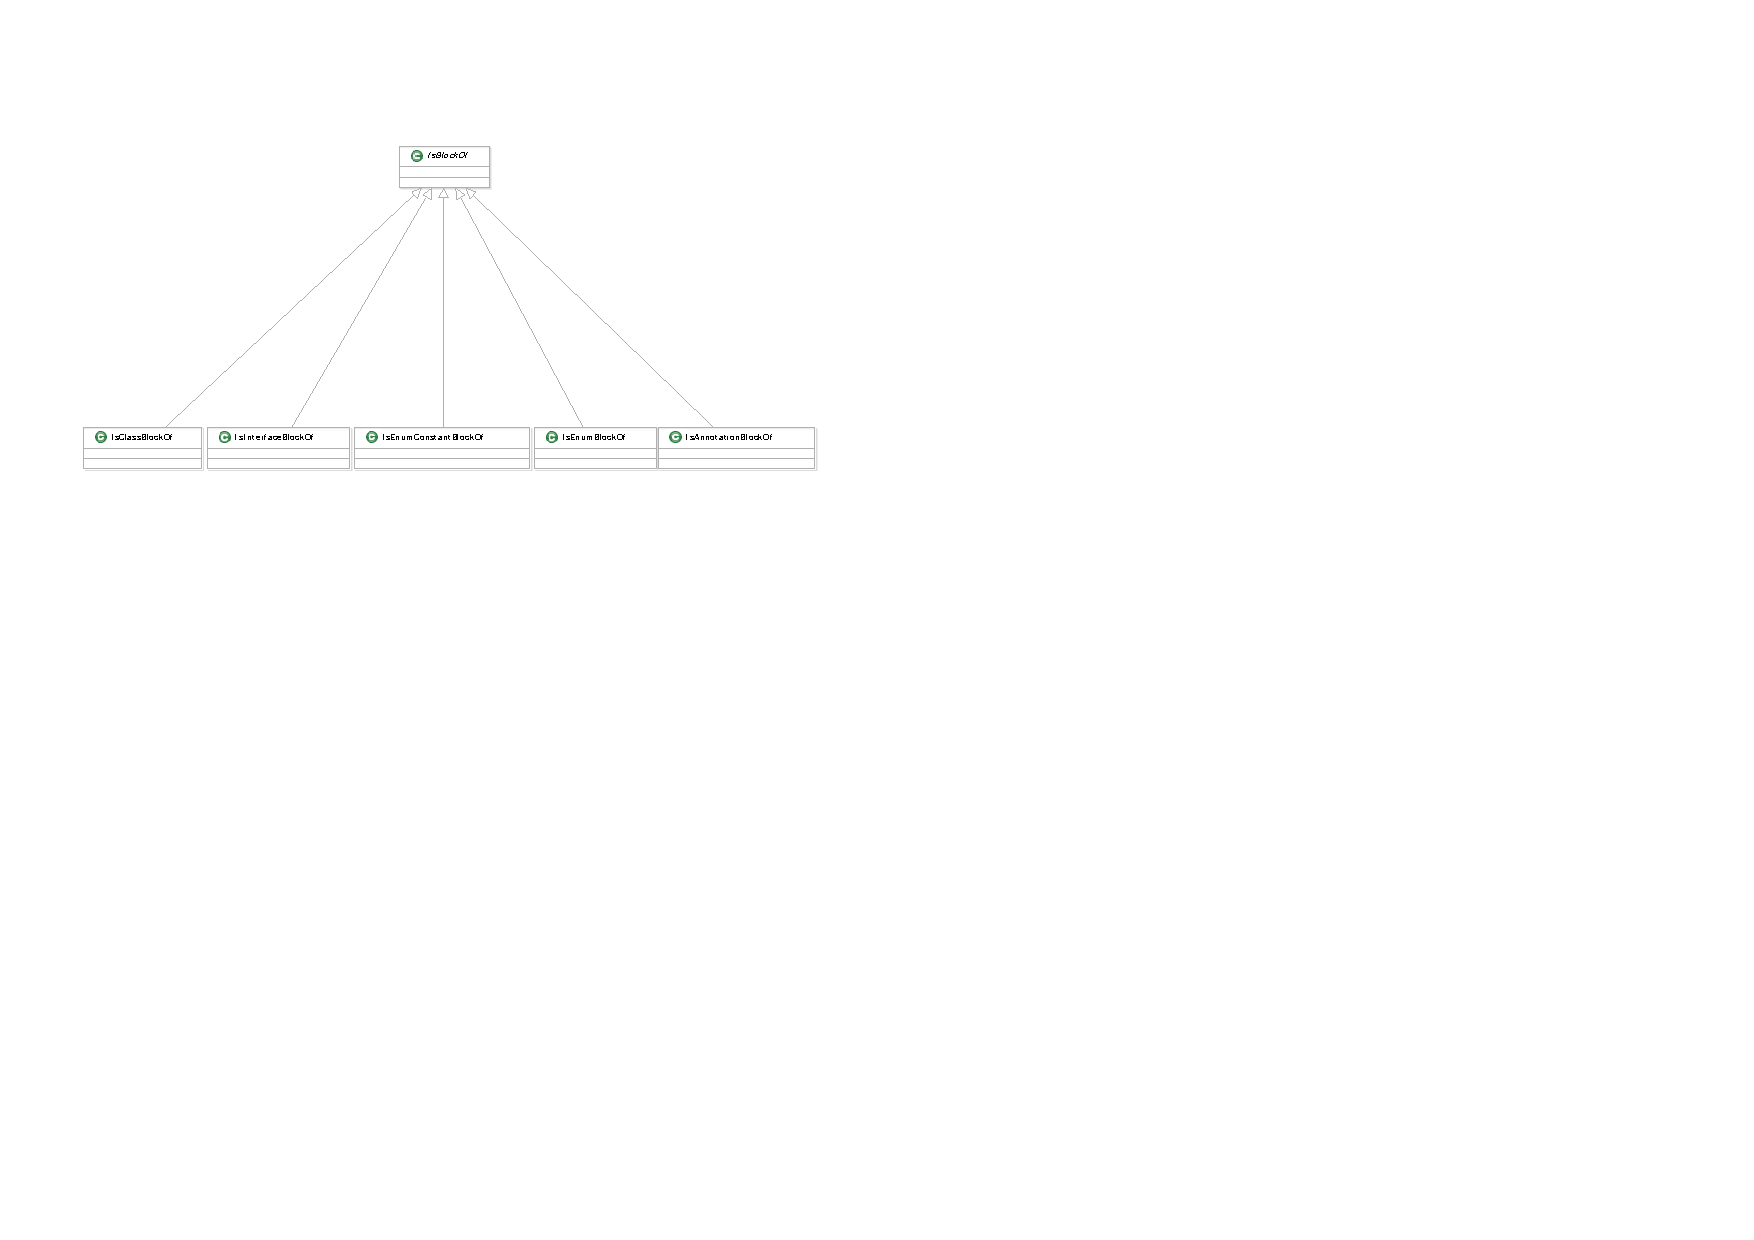
\includegraphics[width=19.8cm, angle=90]{figures/metamodellkanten13.pdf}
	  \caption{Kantentypenhierarchie (Teil 13 / 13)}
  \end{center}
\end{figure}
\clearpage
